
\documentclass[10pt]{article} % For LaTeX2e
% \usepackage{tmlr}
% If accepted, instead use the following line for the camera-ready submission:
\usepackage[preprint]{tmlr}
% To de-anonymize and remove mentions to TMLR (for example for posting to preprint servers), instead use the following:
%\usepackage[preprint]{tmlr}

% Optional math commands from https://github.com/goodfeli/dlbook_notation.
%%%%% NEW MATH DEFINITIONS %%%%%

\usepackage{amsmath,amsfonts,bm}

% Mark sections of captions for referring to divisions of figures
\newcommand{\figleft}{{\em (Left)}}
\newcommand{\figcenter}{{\em (Center)}}
\newcommand{\figright}{{\em (Right)}}
\newcommand{\figtop}{{\em (Top)}}
\newcommand{\figbottom}{{\em (Bottom)}}
\newcommand{\captiona}{{\em (a)}}
\newcommand{\captionb}{{\em (b)}}
\newcommand{\captionc}{{\em (c)}}
\newcommand{\captiond}{{\em (d)}}

% Highlight a newly defined term
\newcommand{\newterm}[1]{{\bf #1}}


% Figure reference, lower-case.
\def\figref#1{figure~\ref{#1}}
% Figure reference, capital. For start of sentence
\def\Figref#1{Figure~\ref{#1}}
\def\twofigref#1#2{figures \ref{#1} and \ref{#2}}
\def\quadfigref#1#2#3#4{figures \ref{#1}, \ref{#2}, \ref{#3} and \ref{#4}}
% Section reference, lower-case.
\def\secref#1{section~\ref{#1}}
% Section reference, capital.
\def\Secref#1{Section~\ref{#1}}
% Reference to two sections.
\def\twosecrefs#1#2{sections \ref{#1} and \ref{#2}}
% Reference to three sections.
\def\secrefs#1#2#3{sections \ref{#1}, \ref{#2} and \ref{#3}}
% Reference to an equation, lower-case.
\def\eqref#1{equation~\ref{#1}}
% Reference to an equation, upper case
\def\Eqref#1{Equation~\ref{#1}}
% A raw reference to an equation---avoid using if possible
\def\plaineqref#1{\ref{#1}}
% Reference to a chapter, lower-case.
\def\chapref#1{chapter~\ref{#1}}
% Reference to an equation, upper case.
\def\Chapref#1{Chapter~\ref{#1}}
% Reference to a range of chapters
\def\rangechapref#1#2{chapters\ref{#1}--\ref{#2}}
% Reference to an algorithm, lower-case.
\def\algref#1{algorithm~\ref{#1}}
% Reference to an algorithm, upper case.
\def\Algref#1{Algorithm~\ref{#1}}
\def\twoalgref#1#2{algorithms \ref{#1} and \ref{#2}}
\def\Twoalgref#1#2{Algorithms \ref{#1} and \ref{#2}}
% Reference to a part, lower case
\def\partref#1{part~\ref{#1}}
% Reference to a part, upper case
\def\Partref#1{Part~\ref{#1}}
\def\twopartref#1#2{parts \ref{#1} and \ref{#2}}

\def\ceil#1{\lceil #1 \rceil}
\def\floor#1{\lfloor #1 \rfloor}
\def\1{\bm{1}}
\newcommand{\train}{\mathcal{D}}
\newcommand{\valid}{\mathcal{D_{\mathrm{valid}}}}
\newcommand{\test}{\mathcal{D_{\mathrm{test}}}}

\def\eps{{\epsilon}}


% Random variables
\def\reta{{\textnormal{$\eta$}}}
\def\ra{{\textnormal{a}}}
\def\rb{{\textnormal{b}}}
\def\rc{{\textnormal{c}}}
\def\rd{{\textnormal{d}}}
\def\re{{\textnormal{e}}}
\def\rf{{\textnormal{f}}}
\def\rg{{\textnormal{g}}}
\def\rh{{\textnormal{h}}}
\def\ri{{\textnormal{i}}}
\def\rj{{\textnormal{j}}}
\def\rk{{\textnormal{k}}}
\def\rl{{\textnormal{l}}}
% rm is already a command, just don't name any random variables m
\def\rn{{\textnormal{n}}}
\def\ro{{\textnormal{o}}}
\def\rp{{\textnormal{p}}}
\def\rq{{\textnormal{q}}}
\def\rr{{\textnormal{r}}}
\def\rs{{\textnormal{s}}}
\def\rt{{\textnormal{t}}}
\def\ru{{\textnormal{u}}}
\def\rv{{\textnormal{v}}}
\def\rw{{\textnormal{w}}}
\def\rx{{\textnormal{x}}}
\def\ry{{\textnormal{y}}}
\def\rz{{\textnormal{z}}}

% Random vectors
\def\rvepsilon{{\mathbf{\epsilon}}}
\def\rvtheta{{\mathbf{\theta}}}
\def\rva{{\mathbf{a}}}
\def\rvb{{\mathbf{b}}}
\def\rvc{{\mathbf{c}}}
\def\rvd{{\mathbf{d}}}
\def\rve{{\mathbf{e}}}
\def\rvf{{\mathbf{f}}}
\def\rvg{{\mathbf{g}}}
\def\rvh{{\mathbf{h}}}
\def\rvu{{\mathbf{i}}}
\def\rvj{{\mathbf{j}}}
\def\rvk{{\mathbf{k}}}
\def\rvl{{\mathbf{l}}}
\def\rvm{{\mathbf{m}}}
\def\rvn{{\mathbf{n}}}
\def\rvo{{\mathbf{o}}}
\def\rvp{{\mathbf{p}}}
\def\rvq{{\mathbf{q}}}
\def\rvr{{\mathbf{r}}}
\def\rvs{{\mathbf{s}}}
\def\rvt{{\mathbf{t}}}
\def\rvu{{\mathbf{u}}}
\def\rvv{{\mathbf{v}}}
\def\rvw{{\mathbf{w}}}
\def\rvx{{\mathbf{x}}}
\def\rvy{{\mathbf{y}}}
\def\rvz{{\mathbf{z}}}

% Elements of random vectors
\def\erva{{\textnormal{a}}}
\def\ervb{{\textnormal{b}}}
\def\ervc{{\textnormal{c}}}
\def\ervd{{\textnormal{d}}}
\def\erve{{\textnormal{e}}}
\def\ervf{{\textnormal{f}}}
\def\ervg{{\textnormal{g}}}
\def\ervh{{\textnormal{h}}}
\def\ervi{{\textnormal{i}}}
\def\ervj{{\textnormal{j}}}
\def\ervk{{\textnormal{k}}}
\def\ervl{{\textnormal{l}}}
\def\ervm{{\textnormal{m}}}
\def\ervn{{\textnormal{n}}}
\def\ervo{{\textnormal{o}}}
\def\ervp{{\textnormal{p}}}
\def\ervq{{\textnormal{q}}}
\def\ervr{{\textnormal{r}}}
\def\ervs{{\textnormal{s}}}
\def\ervt{{\textnormal{t}}}
\def\ervu{{\textnormal{u}}}
\def\ervv{{\textnormal{v}}}
\def\ervw{{\textnormal{w}}}
\def\ervx{{\textnormal{x}}}
\def\ervy{{\textnormal{y}}}
\def\ervz{{\textnormal{z}}}

% Random matrices
\def\rmA{{\mathbf{A}}}
\def\rmB{{\mathbf{B}}}
\def\rmC{{\mathbf{C}}}
\def\rmD{{\mathbf{D}}}
\def\rmE{{\mathbf{E}}}
\def\rmF{{\mathbf{F}}}
\def\rmG{{\mathbf{G}}}
\def\rmH{{\mathbf{H}}}
\def\rmI{{\mathbf{I}}}
\def\rmJ{{\mathbf{J}}}
\def\rmK{{\mathbf{K}}}
\def\rmL{{\mathbf{L}}}
\def\rmM{{\mathbf{M}}}
\def\rmN{{\mathbf{N}}}
\def\rmO{{\mathbf{O}}}
\def\rmP{{\mathbf{P}}}
\def\rmQ{{\mathbf{Q}}}
\def\rmR{{\mathbf{R}}}
\def\rmS{{\mathbf{S}}}
\def\rmT{{\mathbf{T}}}
\def\rmU{{\mathbf{U}}}
\def\rmV{{\mathbf{V}}}
\def\rmW{{\mathbf{W}}}
\def\rmX{{\mathbf{X}}}
\def\rmY{{\mathbf{Y}}}
\def\rmZ{{\mathbf{Z}}}

% Elements of random matrices
\def\ermA{{\textnormal{A}}}
\def\ermB{{\textnormal{B}}}
\def\ermC{{\textnormal{C}}}
\def\ermD{{\textnormal{D}}}
\def\ermE{{\textnormal{E}}}
\def\ermF{{\textnormal{F}}}
\def\ermG{{\textnormal{G}}}
\def\ermH{{\textnormal{H}}}
\def\ermI{{\textnormal{I}}}
\def\ermJ{{\textnormal{J}}}
\def\ermK{{\textnormal{K}}}
\def\ermL{{\textnormal{L}}}
\def\ermM{{\textnormal{M}}}
\def\ermN{{\textnormal{N}}}
\def\ermO{{\textnormal{O}}}
\def\ermP{{\textnormal{P}}}
\def\ermQ{{\textnormal{Q}}}
\def\ermR{{\textnormal{R}}}
\def\ermS{{\textnormal{S}}}
\def\ermT{{\textnormal{T}}}
\def\ermU{{\textnormal{U}}}
\def\ermV{{\textnormal{V}}}
\def\ermW{{\textnormal{W}}}
\def\ermX{{\textnormal{X}}}
\def\ermY{{\textnormal{Y}}}
\def\ermZ{{\textnormal{Z}}}

% Vectors
\def\vzero{{\bm{0}}}
\def\vone{{\bm{1}}}
\def\vmu{{\bm{\mu}}}
\def\vtheta{{\bm{\theta}}}
\def\va{{\bm{a}}}
\def\vb{{\bm{b}}}
\def\vc{{\bm{c}}}
\def\vd{{\bm{d}}}
\def\ve{{\bm{e}}}
\def\vf{{\bm{f}}}
\def\vg{{\bm{g}}}
\def\vh{{\bm{h}}}
\def\vi{{\bm{i}}}
\def\vj{{\bm{j}}}
\def\vk{{\bm{k}}}
\def\vl{{\bm{l}}}
\def\vm{{\bm{m}}}
\def\vn{{\bm{n}}}
\def\vo{{\bm{o}}}
\def\vp{{\bm{p}}}
\def\vq{{\bm{q}}}
\def\vr{{\bm{r}}}
\def\vs{{\bm{s}}}
\def\vt{{\bm{t}}}
\def\vu{{\bm{u}}}
\def\vv{{\bm{v}}}
\def\vw{{\bm{w}}}
\def\vx{{\bm{x}}}
\def\vy{{\bm{y}}}
\def\vz{{\bm{z}}}

% Elements of vectors
\def\evalpha{{\alpha}}
\def\evbeta{{\beta}}
\def\evepsilon{{\epsilon}}
\def\evlambda{{\lambda}}
\def\evomega{{\omega}}
\def\evmu{{\mu}}
\def\evpsi{{\psi}}
\def\evsigma{{\sigma}}
\def\evtheta{{\theta}}
\def\eva{{a}}
\def\evb{{b}}
\def\evc{{c}}
\def\evd{{d}}
\def\eve{{e}}
\def\evf{{f}}
\def\evg{{g}}
\def\evh{{h}}
\def\evi{{i}}
\def\evj{{j}}
\def\evk{{k}}
\def\evl{{l}}
\def\evm{{m}}
\def\evn{{n}}
\def\evo{{o}}
\def\evp{{p}}
\def\evq{{q}}
\def\evr{{r}}
\def\evs{{s}}
\def\evt{{t}}
\def\evu{{u}}
\def\evv{{v}}
\def\evw{{w}}
\def\evx{{x}}
\def\evy{{y}}
\def\evz{{z}}

% Matrix
\def\mA{{\bm{A}}}
\def\mB{{\bm{B}}}
\def\mC{{\bm{C}}}
\def\mD{{\bm{D}}}
\def\mE{{\bm{E}}}
\def\mF{{\bm{F}}}
\def\mG{{\bm{G}}}
\def\mH{{\bm{H}}}
\def\mI{{\bm{I}}}
\def\mJ{{\bm{J}}}
\def\mK{{\bm{K}}}
\def\mL{{\bm{L}}}
\def\mM{{\bm{M}}}
\def\mN{{\bm{N}}}
\def\mO{{\bm{O}}}
\def\mP{{\bm{P}}}
\def\mQ{{\bm{Q}}}
\def\mR{{\bm{R}}}
\def\mS{{\bm{S}}}
\def\mT{{\bm{T}}}
\def\mU{{\bm{U}}}
\def\mV{{\bm{V}}}
\def\mW{{\bm{W}}}
\def\mX{{\bm{X}}}
\def\mY{{\bm{Y}}}
\def\mZ{{\bm{Z}}}
\def\mBeta{{\bm{\beta}}}
\def\mPhi{{\bm{\Phi}}}
\def\mLambda{{\bm{\Lambda}}}
\def\mSigma{{\bm{\Sigma}}}

% Tensor
\DeclareMathAlphabet{\mathsfit}{\encodingdefault}{\sfdefault}{m}{sl}
\SetMathAlphabet{\mathsfit}{bold}{\encodingdefault}{\sfdefault}{bx}{n}
\newcommand{\tens}[1]{\bm{\mathsfit{#1}}}
\def\tA{{\tens{A}}}
\def\tB{{\tens{B}}}
\def\tC{{\tens{C}}}
\def\tD{{\tens{D}}}
\def\tE{{\tens{E}}}
\def\tF{{\tens{F}}}
\def\tG{{\tens{G}}}
\def\tH{{\tens{H}}}
\def\tI{{\tens{I}}}
\def\tJ{{\tens{J}}}
\def\tK{{\tens{K}}}
\def\tL{{\tens{L}}}
\def\tM{{\tens{M}}}
\def\tN{{\tens{N}}}
\def\tO{{\tens{O}}}
\def\tP{{\tens{P}}}
\def\tQ{{\tens{Q}}}
\def\tR{{\tens{R}}}
\def\tS{{\tens{S}}}
\def\tT{{\tens{T}}}
\def\tU{{\tens{U}}}
\def\tV{{\tens{V}}}
\def\tW{{\tens{W}}}
\def\tX{{\tens{X}}}
\def\tY{{\tens{Y}}}
\def\tZ{{\tens{Z}}}


% Graph
\def\gA{{\mathcal{A}}}
\def\gB{{\mathcal{B}}}
\def\gC{{\mathcal{C}}}
\def\gD{{\mathcal{D}}}
\def\gE{{\mathcal{E}}}
\def\gF{{\mathcal{F}}}
\def\gG{{\mathcal{G}}}
\def\gH{{\mathcal{H}}}
\def\gI{{\mathcal{I}}}
\def\gJ{{\mathcal{J}}}
\def\gK{{\mathcal{K}}}
\def\gL{{\mathcal{L}}}
\def\gM{{\mathcal{M}}}
\def\gN{{\mathcal{N}}}
\def\gO{{\mathcal{O}}}
\def\gP{{\mathcal{P}}}
\def\gQ{{\mathcal{Q}}}
\def\gR{{\mathcal{R}}}
\def\gS{{\mathcal{S}}}
\def\gT{{\mathcal{T}}}
\def\gU{{\mathcal{U}}}
\def\gV{{\mathcal{V}}}
\def\gW{{\mathcal{W}}}
\def\gX{{\mathcal{X}}}
\def\gY{{\mathcal{Y}}}
\def\gZ{{\mathcal{Z}}}

% Sets
\def\sA{{\mathbb{A}}}
\def\sB{{\mathbb{B}}}
\def\sC{{\mathbb{C}}}
\def\sD{{\mathbb{D}}}
% Don't use a set called E, because this would be the same as our symbol
% for expectation.
\def\sF{{\mathbb{F}}}
\def\sG{{\mathbb{G}}}
\def\sH{{\mathbb{H}}}
\def\sI{{\mathbb{I}}}
\def\sJ{{\mathbb{J}}}
\def\sK{{\mathbb{K}}}
\def\sL{{\mathbb{L}}}
\def\sM{{\mathbb{M}}}
\def\sN{{\mathbb{N}}}
\def\sO{{\mathbb{O}}}
\def\sP{{\mathbb{P}}}
\def\sQ{{\mathbb{Q}}}
\def\sR{{\mathbb{R}}}
\def\sS{{\mathbb{S}}}
\def\sT{{\mathbb{T}}}
\def\sU{{\mathbb{U}}}
\def\sV{{\mathbb{V}}}
\def\sW{{\mathbb{W}}}
\def\sX{{\mathbb{X}}}
\def\sY{{\mathbb{Y}}}
\def\sZ{{\mathbb{Z}}}

% Entries of a matrix
\def\emLambda{{\Lambda}}
\def\emA{{A}}
\def\emB{{B}}
\def\emC{{C}}
\def\emD{{D}}
\def\emE{{E}}
\def\emF{{F}}
\def\emG{{G}}
\def\emH{{H}}
\def\emI{{I}}
\def\emJ{{J}}
\def\emK{{K}}
\def\emL{{L}}
\def\emM{{M}}
\def\emN{{N}}
\def\emO{{O}}
\def\emP{{P}}
\def\emQ{{Q}}
\def\emR{{R}}
\def\emS{{S}}
\def\emT{{T}}
\def\emU{{U}}
\def\emV{{V}}
\def\emW{{W}}
\def\emX{{X}}
\def\emY{{Y}}
\def\emZ{{Z}}
\def\emSigma{{\Sigma}}

% entries of a tensor
% Same font as tensor, without \bm wrapper
\newcommand{\etens}[1]{\mathsfit{#1}}
\def\etLambda{{\etens{\Lambda}}}
\def\etA{{\etens{A}}}
\def\etB{{\etens{B}}}
\def\etC{{\etens{C}}}
\def\etD{{\etens{D}}}
\def\etE{{\etens{E}}}
\def\etF{{\etens{F}}}
\def\etG{{\etens{G}}}
\def\etH{{\etens{H}}}
\def\etI{{\etens{I}}}
\def\etJ{{\etens{J}}}
\def\etK{{\etens{K}}}
\def\etL{{\etens{L}}}
\def\etM{{\etens{M}}}
\def\etN{{\etens{N}}}
\def\etO{{\etens{O}}}
\def\etP{{\etens{P}}}
\def\etQ{{\etens{Q}}}
\def\etR{{\etens{R}}}
\def\etS{{\etens{S}}}
\def\etT{{\etens{T}}}
\def\etU{{\etens{U}}}
\def\etV{{\etens{V}}}
\def\etW{{\etens{W}}}
\def\etX{{\etens{X}}}
\def\etY{{\etens{Y}}}
\def\etZ{{\etens{Z}}}

% The true underlying data generating distribution
\newcommand{\pdata}{p_{\rm{data}}}
% The empirical distribution defined by the training set
\newcommand{\ptrain}{\hat{p}_{\rm{data}}}
\newcommand{\Ptrain}{\hat{P}_{\rm{data}}}
% The model distribution
\newcommand{\pmodel}{p_{\rm{model}}}
\newcommand{\Pmodel}{P_{\rm{model}}}
\newcommand{\ptildemodel}{\tilde{p}_{\rm{model}}}
% Stochastic autoencoder distributions
\newcommand{\pencode}{p_{\rm{encoder}}}
\newcommand{\pdecode}{p_{\rm{decoder}}}
\newcommand{\precons}{p_{\rm{reconstruct}}}

\newcommand{\laplace}{\mathrm{Laplace}} % Laplace distribution

\newcommand{\E}{\mathbb{E}}
\newcommand{\Ls}{\mathcal{L}}
\newcommand{\R}{\mathbb{R}}
\newcommand{\emp}{\tilde{p}}
\newcommand{\lr}{\alpha}
\newcommand{\reg}{\lambda}
\newcommand{\rect}{\mathrm{rectifier}}
\newcommand{\softmax}{\mathrm{softmax}}
\newcommand{\sigmoid}{\sigma}
\newcommand{\softplus}{\zeta}
\newcommand{\KL}{D_{\mathrm{KL}}}
\newcommand{\Var}{\mathrm{Var}}
\newcommand{\standarderror}{\mathrm{SE}}
\newcommand{\Cov}{\mathrm{Cov}}
% Wolfram Mathworld says $L^2$ is for function spaces and $\ell^2$ is for vectors
% But then they seem to use $L^2$ for vectors throughout the site, and so does
% wikipedia.
\newcommand{\normlzero}{L^0}
\newcommand{\normlone}{L^1}
\newcommand{\normltwo}{L^2}
\newcommand{\normlp}{L^p}
\newcommand{\normmax}{L^\infty}

\newcommand{\parents}{Pa} % See usage in notation.tex. Chosen to match Daphne's book.

\DeclareMathOperator*{\argmax}{arg\,max}
\DeclareMathOperator*{\argmin}{arg\,min}

\DeclareMathOperator{\sign}{sign}
\DeclareMathOperator{\Tr}{Tr}
\let\ab\allowbreak


\usepackage{hyperref}
\usepackage{url}
\usepackage{amsthm}
\usepackage{graphicx}
\usepackage{minted}


\newtheorem{theorem}{Theorem}
\newtheorem*{remark}{Remark}


\title{A simple, fast, and reliable method for PMF estimation from samples}

% Authors must not appear in the submitted version. They should be hidden
% as long as the tmlr package is used without the [accepted] or [preprint] options.
% Non-anonymous submissions will be rejected without review.

\author{\name Alex Shtoff \email alexander.shtoff@tii.ae \\ Technology Innovation Institute\\}
% \author{\name Alex Shtoff \email alex.shtof@gmail.com}

% The \author macro works with any number of authors. Use \AND 
% to separate the names and addresses of multiple authors.

\newcommand{\fix}{\marginpar{FIX}}
\newcommand{\new}{\marginpar{NEW}}

\newminted[pycode]{python}{tabsize=4, fontsize=\scriptsize, frame=lines, framesep=\fboxsep, rulecolor=\color{gray!40}}

\def\month{MM}  % Insert correct month for camera-ready version
\def\year{YYYY} % Insert correct year for camera-ready version
\def\openreview{\url{https://openreview.net/forum?id=XXXX}} % Insert correct link to OpenReview for camera-ready version

\DeclareMathOperator{\diag}{diag}

\begin{document}


\maketitle

\begin{abstract}
We introduce a \emph{simple}, \emph{fast}, and \emph{reliable} non-parametric method to obtain a smooth estimate of a probability mass function (PMF) on $[N] = \{0,1, \dots, N - 1\}$. The core idea is to treat the empirical counts as a signal on a line graph and apply a data-dependent low-pass filter. Concretely, we form a symmetric tri-diagonal operator $\mH = \mL - \diag(\vv)$—the path graph Laplacian $\mL$ plus a diagonal bias $\vv$ built from the empirical counts—and then keep only the first $k$ eigenvectors, corresponding to the smallest eigenvalues. Projecting the empirical histogram onto this $k$-dimensional subspace produces a smooth, multi-modal estimate that preserves coarse structure while suppressing noise. A light post-processing step of clipping and re-normalizing produces a valid PMF. 

Since our main computational workhorse is computing eigenpairs of a symmetric tridiagonal matrix, we stand on the shoulders of the giants who devised and implemented fast and extremely reliable solvers that run in $O(kN)$ time and $O(N)$ memory for a PMF over $[N]$. Thus, our method scales linearly with $N$ and $k$, and requires no monitoring and almost no tuning. Our aim are applications that require a rough estimate of the PMF, while being reliable enough to ``just work'', such as visualization by data scientists, or feature engineering with automated pipelines that run without human intervention at all.

\end{abstract}

\section{Introduction}
Estimating a densities from empirical observations is a fundamental problem with applications ranging from visualizing a histogram to complex generative models for images and text. In this work we focus on an extremely simple and fundamental instance - estimating the density of a discrete random variable with support in $[N] = \{0, 1, 2, \ldots, N - 1\}$ from empirical observations. Our primary focus is on a large $N$, between thousands and a few millions, where the density being estimated is multi-modal and ``heavy tailed'' densities. The quotations are because we do not mean heavy tailedness in the classical sense, due to the finite support, but we do mean that a large portion of their mass is spread far away from a small number of areas of concentration.

Examples include, but not limited to, the well-known power-law distributions, such as the Zipf distributions $p(n)\propto (a+n)^{-b}$, their centered variants $p(n) \propto (a + |n - \mu|)^{-b}$, and their mixtures. Such distributions can be naturally obtained from counts, such as token counts in a corpus of documents in the language domain, or the number of page visits in the recommender systems domain. Moreover, high resolution discretizations of continuous quantities, such as the time since the last user interaction with a given item, product prices, network latencies, or ad auction bids also yield similar density families, since the underlying continuous distributions are typically heavy-tailed. The main feature of the empirical frequency vectors stemming from such distributions is that they are form \emph{noisy} and \emph{sparse} vectors with entries spread throughout, as demonstrated by Figure \ref{fig:distributions}. Indeed, it can be seen that the only distribution whose empirical frequency vectors are different is the \emph{bell shaped} distribution from in the figure, whose samples are mostly concentrated around its (light-tailed) bell. These distributions shall serve as our examples when we analyze the method throughout this paper.

\begin{figure}[tbh]
    \centering
    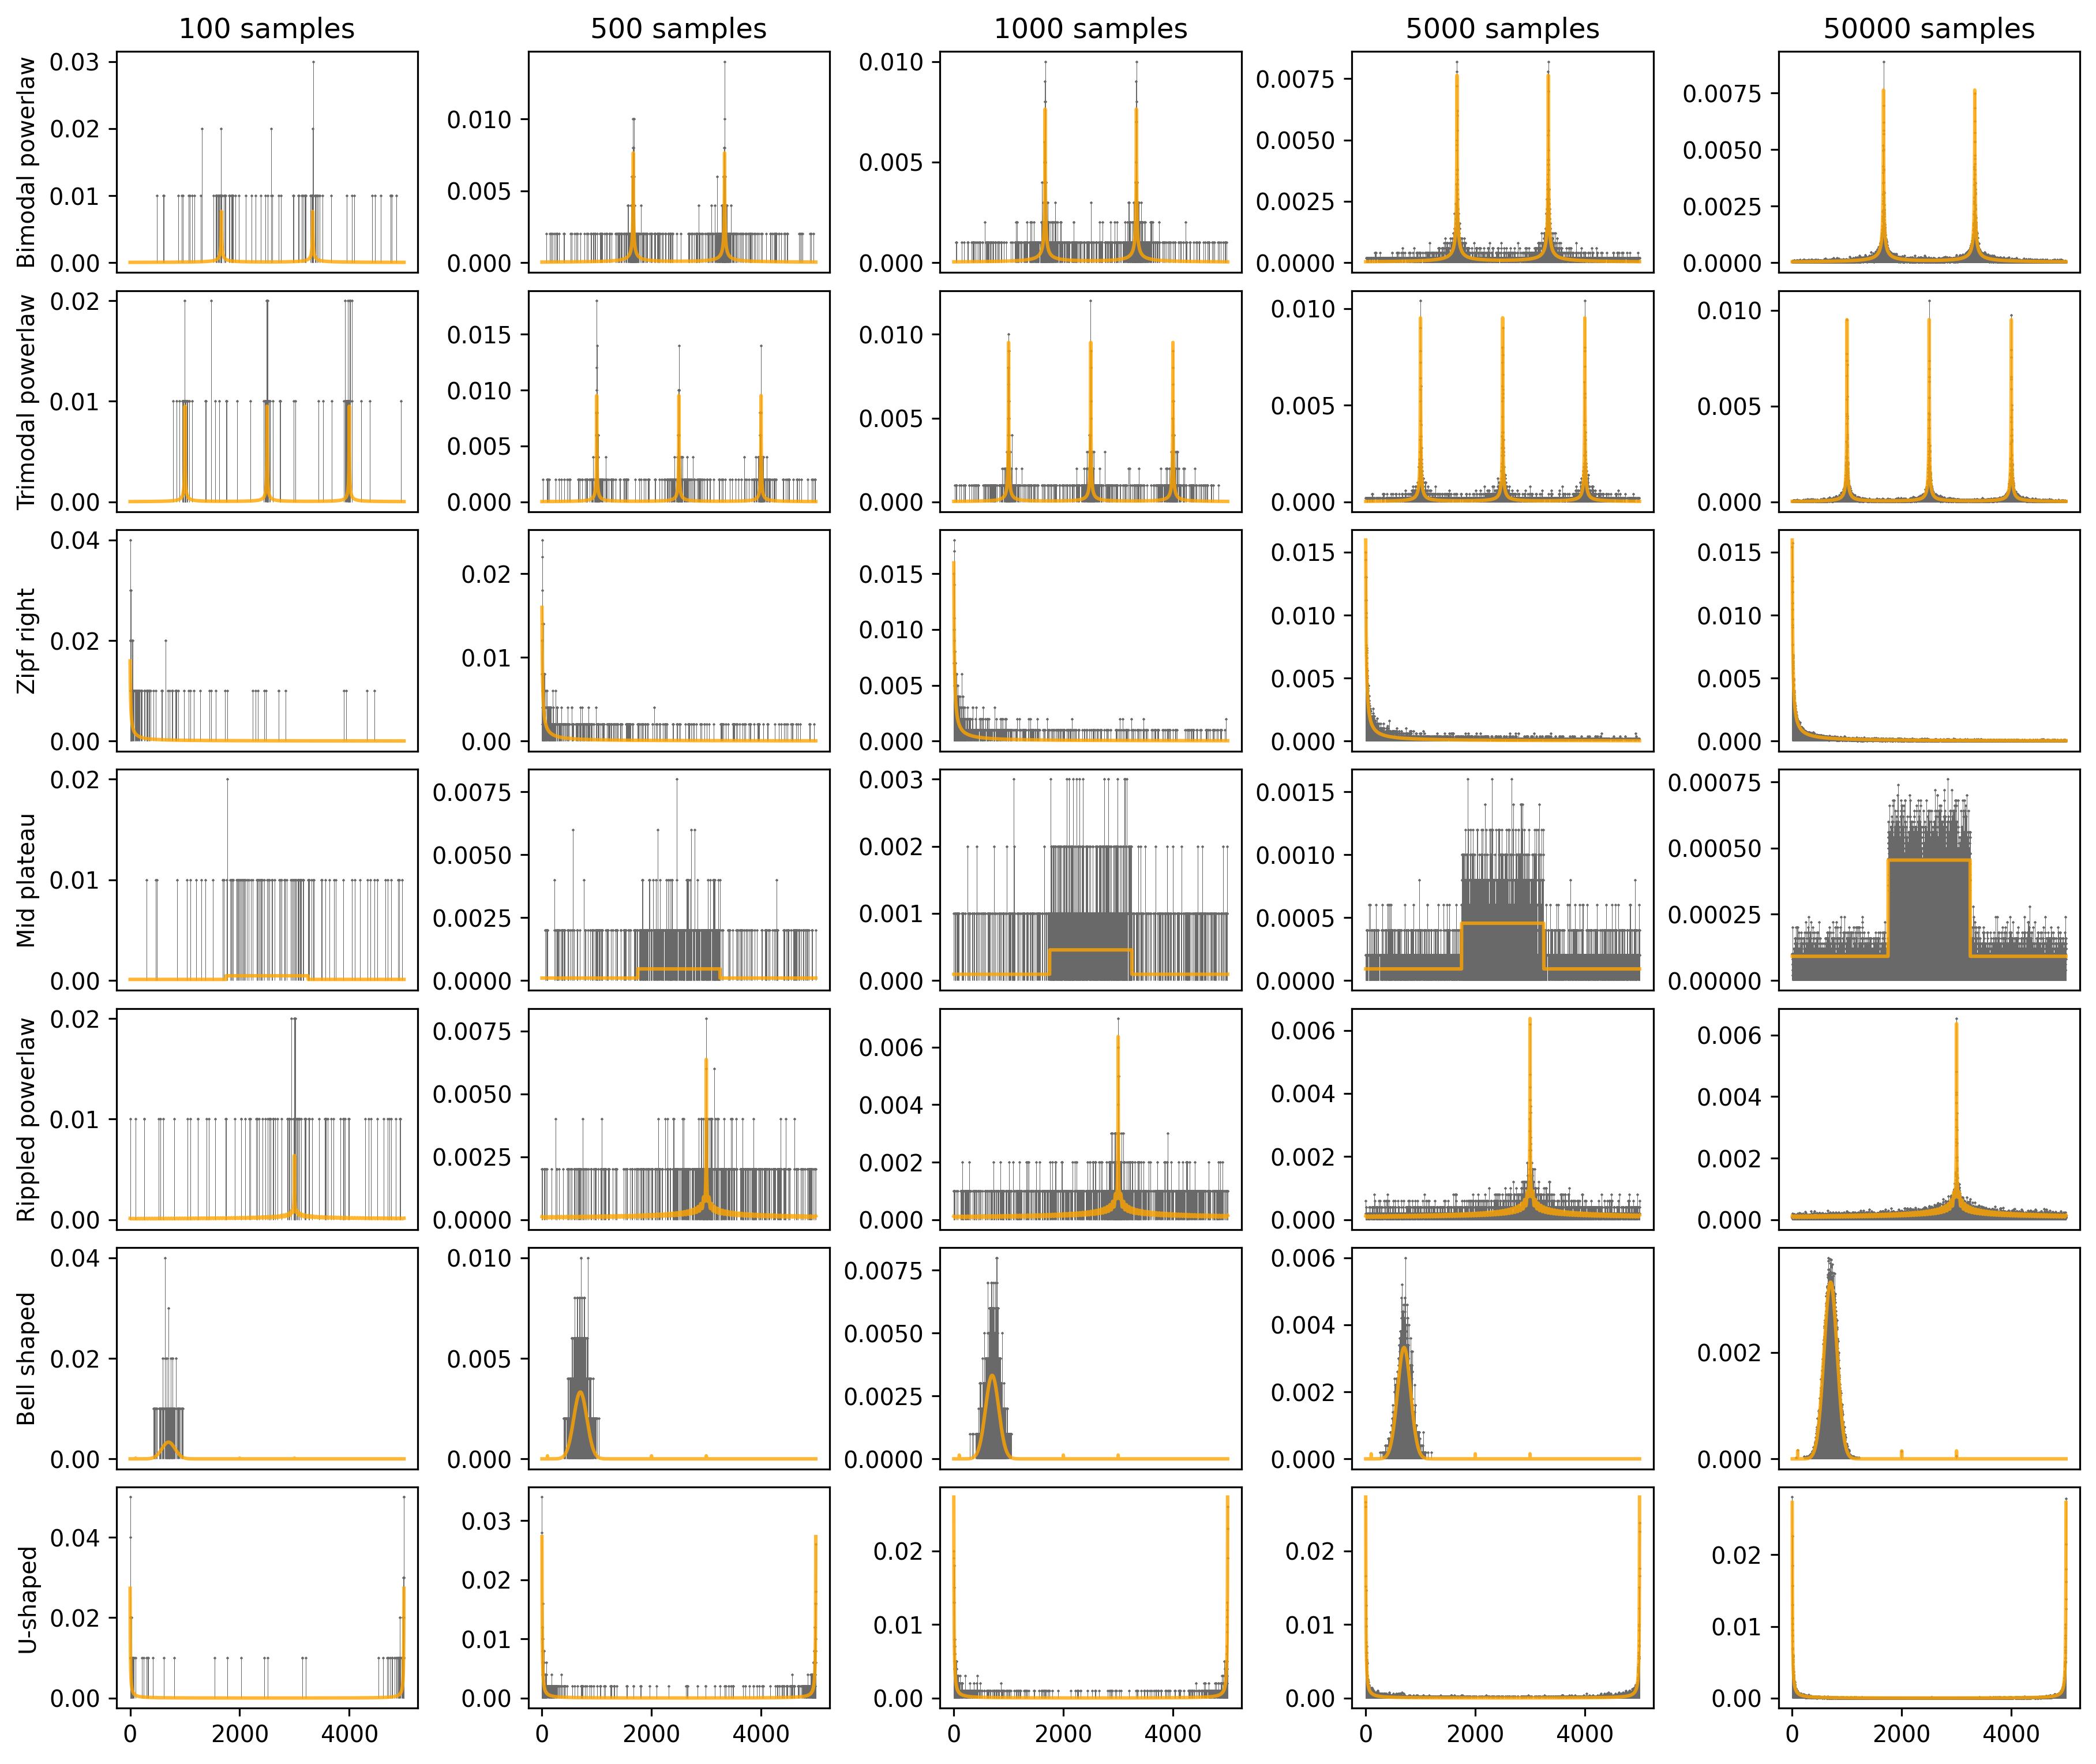
\includegraphics[width=\textwidth]{distributions}
    \caption{Empirical frequency vectors and underlying PMFs that generated them. Orange - true PMF. Gray - empirical frequencies.}
    \label{fig:distributions}
\end{figure}

The three most commonly employed univariate density estimators available in most data analysis software are binned empirical frequencies \citep{binning_pearson},  kernel density estimation \citep{kde_parzen,kde_rosenblatt}, and the logspline methods \citep{KooperbergStone1991,StoneHansenKooperbergTruong1997} implemented in the popular R package having the same name \citep{logsplineCRAN}. The bins and gaussian kernel density estimators are extensively used in standard data visualization libraries, such as Matplotlib \citep{matplotlib} and Seaborn \citep{seaborn}. However, for heavy-tailed distributions it's hard to determine the right placement of bins to get both a reasonable and aesthetically pleasing distribution, whereas with Kernel density estimator one must set the right kernel and its width hyperparameters, which may be challenging and non-intuitive. As we show in our experiments, logspline does prove to be very effective, but occasionally suffers from numerical difficulties and turns out to be slightly less reliable.

We believe that a fundamental and extremely simple problem deserves an extremely simple solution. Thus, our main contribution is a simple, non-parametric, and fast method that fits such heavy-tailed densities well, and is reliable to compute without tuning or oversight. Our main applications in mind are visualization and automated pipelines that need to run without human intervention, such as pipelines for feature engineering in continually-learning recommender systems \citep{offset_adaptive}. Occasionally, we make deliberate design decisions that favor speed, reliability, and simplicity over accuracy and performance. In turns, this yields a reliable method whose implementation is just a few lines of code calling standard reliable linear algebra routines.

After a short literature review in \Secref{sec:review}, we first present our method in \Secref{sec:method}, and demonstrate its strengths and weaknesses with a few synthetic distributions. Then, in \Secref{sec:analysis} we analyze it mathematically, draw a relationship with related methods from other scientific disciplines, and motivate the meaning of its only hyperparameter, the number of eigen-pairs, as an upper bound on the expected number of modes. The somewhat nonstandard structure, where we show results of experiments on synthetic examples outside of a dedicated experiments section was chosen on purpose, since we believe this to be the appropriate way to present our method.

\section{Related work}\label{sec:review}

We situate our approach relative to three strands: (i) classical density/histogram smoothing, (ii) Laplacian and spectral methods for smoothing on graphs, and (iii) Schr\"odinger-type operators obtained by adding a potential to the Laplacian.

\paragraph{Histograms, kernels, and mixtures.} Nonparametric density estimation via kernels goes back to \citet{kde_rosenblatt,kde_parzen}. In practice, both histograms and KDE rely on simple bandwidth/bin-width rules such as those of \citet{Scott1979} and \citet{FreedmanDiaconis1981}, and the averaged shifted histogram provides an inexpensive bridge between histograms and kernels \citep{Scott1985ASH}. A complementary parametric route is finite mixtures, typically fit with the EM algorithm \citep{Dempster1977EM} and surveyed by \citet{McLachlanPeel2000}. . Another widely used alternative is \emph{logspline} density estimation, which models the log-density with cubic splines and selects knots by likelihood-based forward--backward steps; foundational treatments include \citet{KooperbergStone1991,KooperbergStone1992} and the extended spline modeling framework of \citet{StoneHansenKooperbergTruong1997}, with mature implementations such as the R package \emph{logspline} \citep{logsplineCRAN}. Extensions cover binned and spectral settings \citep{Koo2000,KooperbergStoneTruong1995Rate}. These families are effective but introduce tuning - bandwidths, knot numbers/penalties, or component counts and nonconvex fitting - which our goal is to avoid with a parameter-light spectral construction.

\paragraph{Laplacian smoothing and spectral viewpoints.} In computer graphics, Laplacian-based fairing acts as a low-pass smoother \citep{Taubin1995,Desbrun1999ImplicitFairing}. In machine learning, graph-Laplacian regularization underpins manifold learning (Laplacian Eigenmaps, Diffusion Maps), harmonic-field semi-supervised learning, and manifold regularization in RKHS \citep{BelkinNiyogi2003,CoifmanLafon2006,ZhuGhahramaniLafferty2003,BelkinNiyogiSindhwani2006}. A complementary signal-processing perspective advocates spectral filtering and multiscale constructions such as graph wavelets \citep{Shuman2013SPMag,Hammond2011}; for piecewise-smooth targets, $\ell_1$ variants like graph trend filtering provide edge preservation \citep{Wang2016GraphTrendFiltering}. We retain this spectral template but alter the geometry through a data-dependent potential derived from the empirical histogram, which concentrates eigenfunctions near peaks while preserving global regularity.

\paragraph{Laplacians with potentials.} Adding a diagonal potential to the Laplacian yields Schr\"odinger-type operators whose eigenfunctions localize in regions indicated by the potential. \citet{CzajaEhler2013PAMI} introduced \emph{Schr\"odinger Eigenmaps} for semi-supervised learning by incorporating barrier potentials. Our construction instantiates this operator-with-potential principle on a path graph with a potential equal to the empirical histogram, leading to the tridiagonal operator $\mL_{\mathrm{path}} - \diag(\vp)$. Our approach resembles semi-classical signal analysis \citep{semiclassical}, where Schr\"odinger Eigenmaps of a similar nature to ours are used to derive a data dependent basis for signal analysis for pulse-like signals, such as heart-rate. Smoothing is then obtained by truncating its spectrum. The resulting procedure keeps a linear spectral pipeline and limits hyperparameters to the number of retained modes, while adapting the basis to observed mass (contrasting with bandwidth and component-count selection in KDE/mixtures and the penalty choices and nonsmooth solvers of $\ell_1$ graph smoothers). Our work can be seen as a direct application of these approaches to sparse noisy empirical frequency vectors whose underlying PMF has a pulse-like shape, with slight adaptations. In fact, the idea of obtaining a PMF estimate by projecting onto an orthogonal basis dates back to \citet{cencov1962estimation}, and our method is just a variant with Schr\"odinger Eigenmaps being the orthogonal basis of choice, instead of a data independent basis.

\section{Our method}\label{sec:method}
To describe our method, we denote by $\Delta_N$ the $N$-dimensional probability simplex, by $[x]_+ = \max(x, 0)$ the \emph{relu} function, and by $\mL$ the \emph{Laplacian} matrix
\begin{equation}\label{eq:laplacian}
\mL =\begin{pmatrix}
    1 & -1 & 0 & 0 & \cdots & 0 \\
    -1 & 2 & -1 & 0 & \cdots & 0 \\
    0 & -1 & 2 & -1 & \cdots & 0 \\
    \vdots & \vdots & \ddots & \ddots & \ddots & \vdots \\
    0 & 0 & \cdots & -1 & 2 & -1 \\
    0 & 0 & \cdots & 0 & -1 & 1
    \end{pmatrix},
\end{equation}
which lies at the heart of our method. Note, that $\mL$ is symmetric and tridiagonal.

Having observed samples from $[N]$, the inputs to our method are the vector $\vp \in \Delta_N$ of the empirical sample frequencies, and a small integer $k \in \sN$, e.g., $k = 10$. The method consists of the following four steps:
\begin{enumerate}
\item Form the symmetric and tri-diagonal matrix $\mH = \mL - \diag(\vp)$.
\item Compute the $k$ eigenvectors $\vv_1, \dots, \vv_k$ corresponding to the \emph{smallest} eigenvalues of $\mH$, and place them in the columns of the matrix $\mV = [\vv_1 \vert \vv_2 \vert \cdots \vert \vv_k]$.
\item Compute $\vu = \mV (\mV^T \vp)$
\item Return the vector $\vq$ with $\evq_i = [u_i]_+ / \|[\vu]_+ \|_1$.
\end{enumerate}
At first glance it may not be obvious why those four steps. Readers may notice that that the third step is merely a projection onto the subspace spanned by the eigenvectors, whereas the fourth step is just a normalization. Consequently, the utility of this specific subspace is the main pillar of our method's ability to fit sparse histograms, whereas having the reliable and efficient tools to compute the eigenvectors is the main pillar of our method's efficiency and reliability.

To appreciate the method's simplicity, below is a Python implementing our algorithm:
\begin{pycode}
import numpy as np
import scipy.linalg as la

def estimate_pmf(samples, k=10):
    # compute empirical frequencies
    p = np.bincount(samples, minlength=np.max(samples) + 1)
    p = p.astype(float) / np.sum(p)

    # Form the diagonals of H
    diag_l = np.r_[1, np.full(p.size - 2, 2), 1]  # [1, 2, ..., 2, 1]
    diag_h = diag_l - p
    off_diag_h = np.full(p.size - 1, -1)          # [-1, ..., -1]

    # compute first k eigenvectors of H
    _, v = la.eigh_tridiagonal(diag_h, off_diag_h, select="i", select_range=(0, k - 1))

    # project and normalize
    u = v @ (v.T @ p)
    return np.maximum(u, 0) / np.sum(np.maximum(u, 0))
\end{pycode}

But before taking a closer look, we would like to draw the readers' attention to Figure \ref{fig:proj_500_samples}, where we demonstrate using synthetic examples where our method shines versus where it does not. It is apparent that ``spiky'' distributions having significant mass both around their modes but also far away are fit well, whereas Gaussian kernel-density estimation falls short. Our method is slighly less suited to wide bell-shaped distributions, in contrast to Gaussian kernel-density estimation that shines in these cases. Finally, our method performs poorly for discontinuous densities, in contrast to kernel-density estimators that, despite fitting poorly, performs gracefully. Our analysis in the next section attempts to explain these phenomena.

\section{Analysis}\label{sec:analysis}
Although our method is a straightforward instance of Schr\"odinger eigenmaps, and we could simply cite that literature, we present a direct, elementary analysis to offer clearer insight and broader accessibility. We hope that this will inspire similar techniques to be applied to other domains of analyzing univariate data. We rely only on basic linear algebra facts, and offer the viewpoint of optimizing an objective that balances data fitting and regularization, the bread and butter of modern machine learning. Some steps may be routine for readers familiar with related techniques, but this elementary treatment, in our view, makes the key ideas accessible to a much wider audience.

Recall that any real symmetric matrix always has real eigenvalues, and the corresponding eigenvectors form an orthonormal set. A well-known characterization of the eigenvalues and eigenvectors of symmetric matrices is via minimization of quadratic functions. Formally, we have:
\begin{theorem}\label{thm:courant_fischer}
Let $\mA$ be a real symmetric $n \times n$ matrix, let $\lambda_1 \leq \dots \leq\lambda_n$ be its eigenvalues, and let $\ve_1, \dots, \ve_n$ be the corresponding orthonormal eigenvectors. Then,
\[
\ve_k = \argmin_{\vx} \{ \vx^T \mA \vx : \|\vx\|_2 = 1,~\vx^T \ve_1 = 0,~\ldots,~\vx^T \ve_{k-1} = 0 \}.
\]
\end{theorem}
In other words, the eigenvector corresponding to the $k$-th smallest eigenvalue is the unit-norm minimizer the quadratic function $\vx^T \mA \vx$ that is orthogonal to all previous eigenvectors. Even though it is not stated in this form in the literature, this result is typically proved \emph{as a part of} proving the famous Courant-Fischer theorem. See, e.g., the proof of Theorem 4.2.8 in \citet{horn2012matrix}.

Now we shall analyze our method. Consider the matrix $\mH = \mL - \diag(\vp)$, where $\mL$ is the Laplacian defined in \eqref{eq:laplacian}, and $\vp$ is the vector of empirical frequencies. By Theorem \ref{thm:courant_fischer}, the eigenvector corresponding to its smallest eigenvalue minimizes the function
\[
\vx^T (\mL - \diag(\vp)) \vx = \vx^T \mL \vx - \vx^T \diag(\vp) \vx = \underbrace{\vx^T \mL \vx}_{(*)} - \underbrace{\langle \vx^2, \vp \rangle}_{(**)},
\]
where $\vx^2$ denotes component-wise squaring. To grasp the meaning of $(*)$, consider the first-order difference matrix
\[
\mD = \begin{pmatrix}
    1 & -1 & 0 & \dots & 0 \\
    0 & 1 & -1 & \dots & 0 \\
    \vdots &   & \ddots & \ddots \\
    0 & \dots & 0 & 1 & -1
\end{pmatrix}.
\]
It is easy to verify that $\mL = \mD^T \mD$. Therefore,
\[
(*) = \vx^T \mL \vx = \| \mD \vx \|^2,
\]
meaning that this is a smoothness term penalizing the squared-norm of the differences between adjacent components of $\vx$. In other words, it is a \emph{regularizer}, and imposes a non-parametric prior of $\vx$ representing a sequence that changes slowly.

The term $(**)$ is easily recognizable by machine-learning practitioners - it is the widely used inner-product dis-similarity between the vectors $\vx^2$ and $\vp$. It penalizes misalignment between these two vectors, and thus promotes a kind of alignment term between $\vx$ and the empirical frequency vector. 

Intuitively, the first eigenvector just minimizes the balance between these two terms, and thus yields a smooth sequence that captures the overall shape of the density. The second eigenvector aims to minimize the same balance while being orthogonal to the first, thus it may capture additional, more intricate details that were not captured by the first. This pattern repeats for all eigenvectors, each capturing additional details that the previous has not. Consequently, the first $k$ eigenvectors corresponding to the smallest eigenvalues form a dictionary of atoms that is adapted to the distribution being fit.

\Figref{fig:eigenvectors} demonstrates the eigenvectors obtained from samples coming from various synthetic distributions. We can observe empirically that in a multi-modal distribution, the first eigenvector typically captures the most dominant mode: the data alignment term draws the eigenvector towards the mode, whereas the smoothness penalty makes it discard other modes. Having captured all dominant modes, the remaining eigenvectors appear as oscillating sequences with increased frequency, with oscillations mostly concentrating around the modes. Moreover, even though the PMF is noisy and sparse, the eigenvectors appear smooth and close to capturing the over-all shape of the PMF.

This phenomenon is not a coincidence. The eigenvectors of the Laplacian matrix $\mL$ itself are the celebrated Discrete Cosine Transform \citep{the_dct}, which are renowned for their ability to approximate discrete smooth sequences using a linear combination of just a few vectors. In contrast to the discrete cosine transform, which is a data-independent basis, the eigenvectors $\vv_1, \dots, \vv_k$ of the perturbed Laplacian are a \emph{data-dependent} basis for approximating smooth sequences. It concentrates its approximation power in a way that is aligned with the shape of the distribution being fit.

\begin{figure}[tbh]
    \centering
    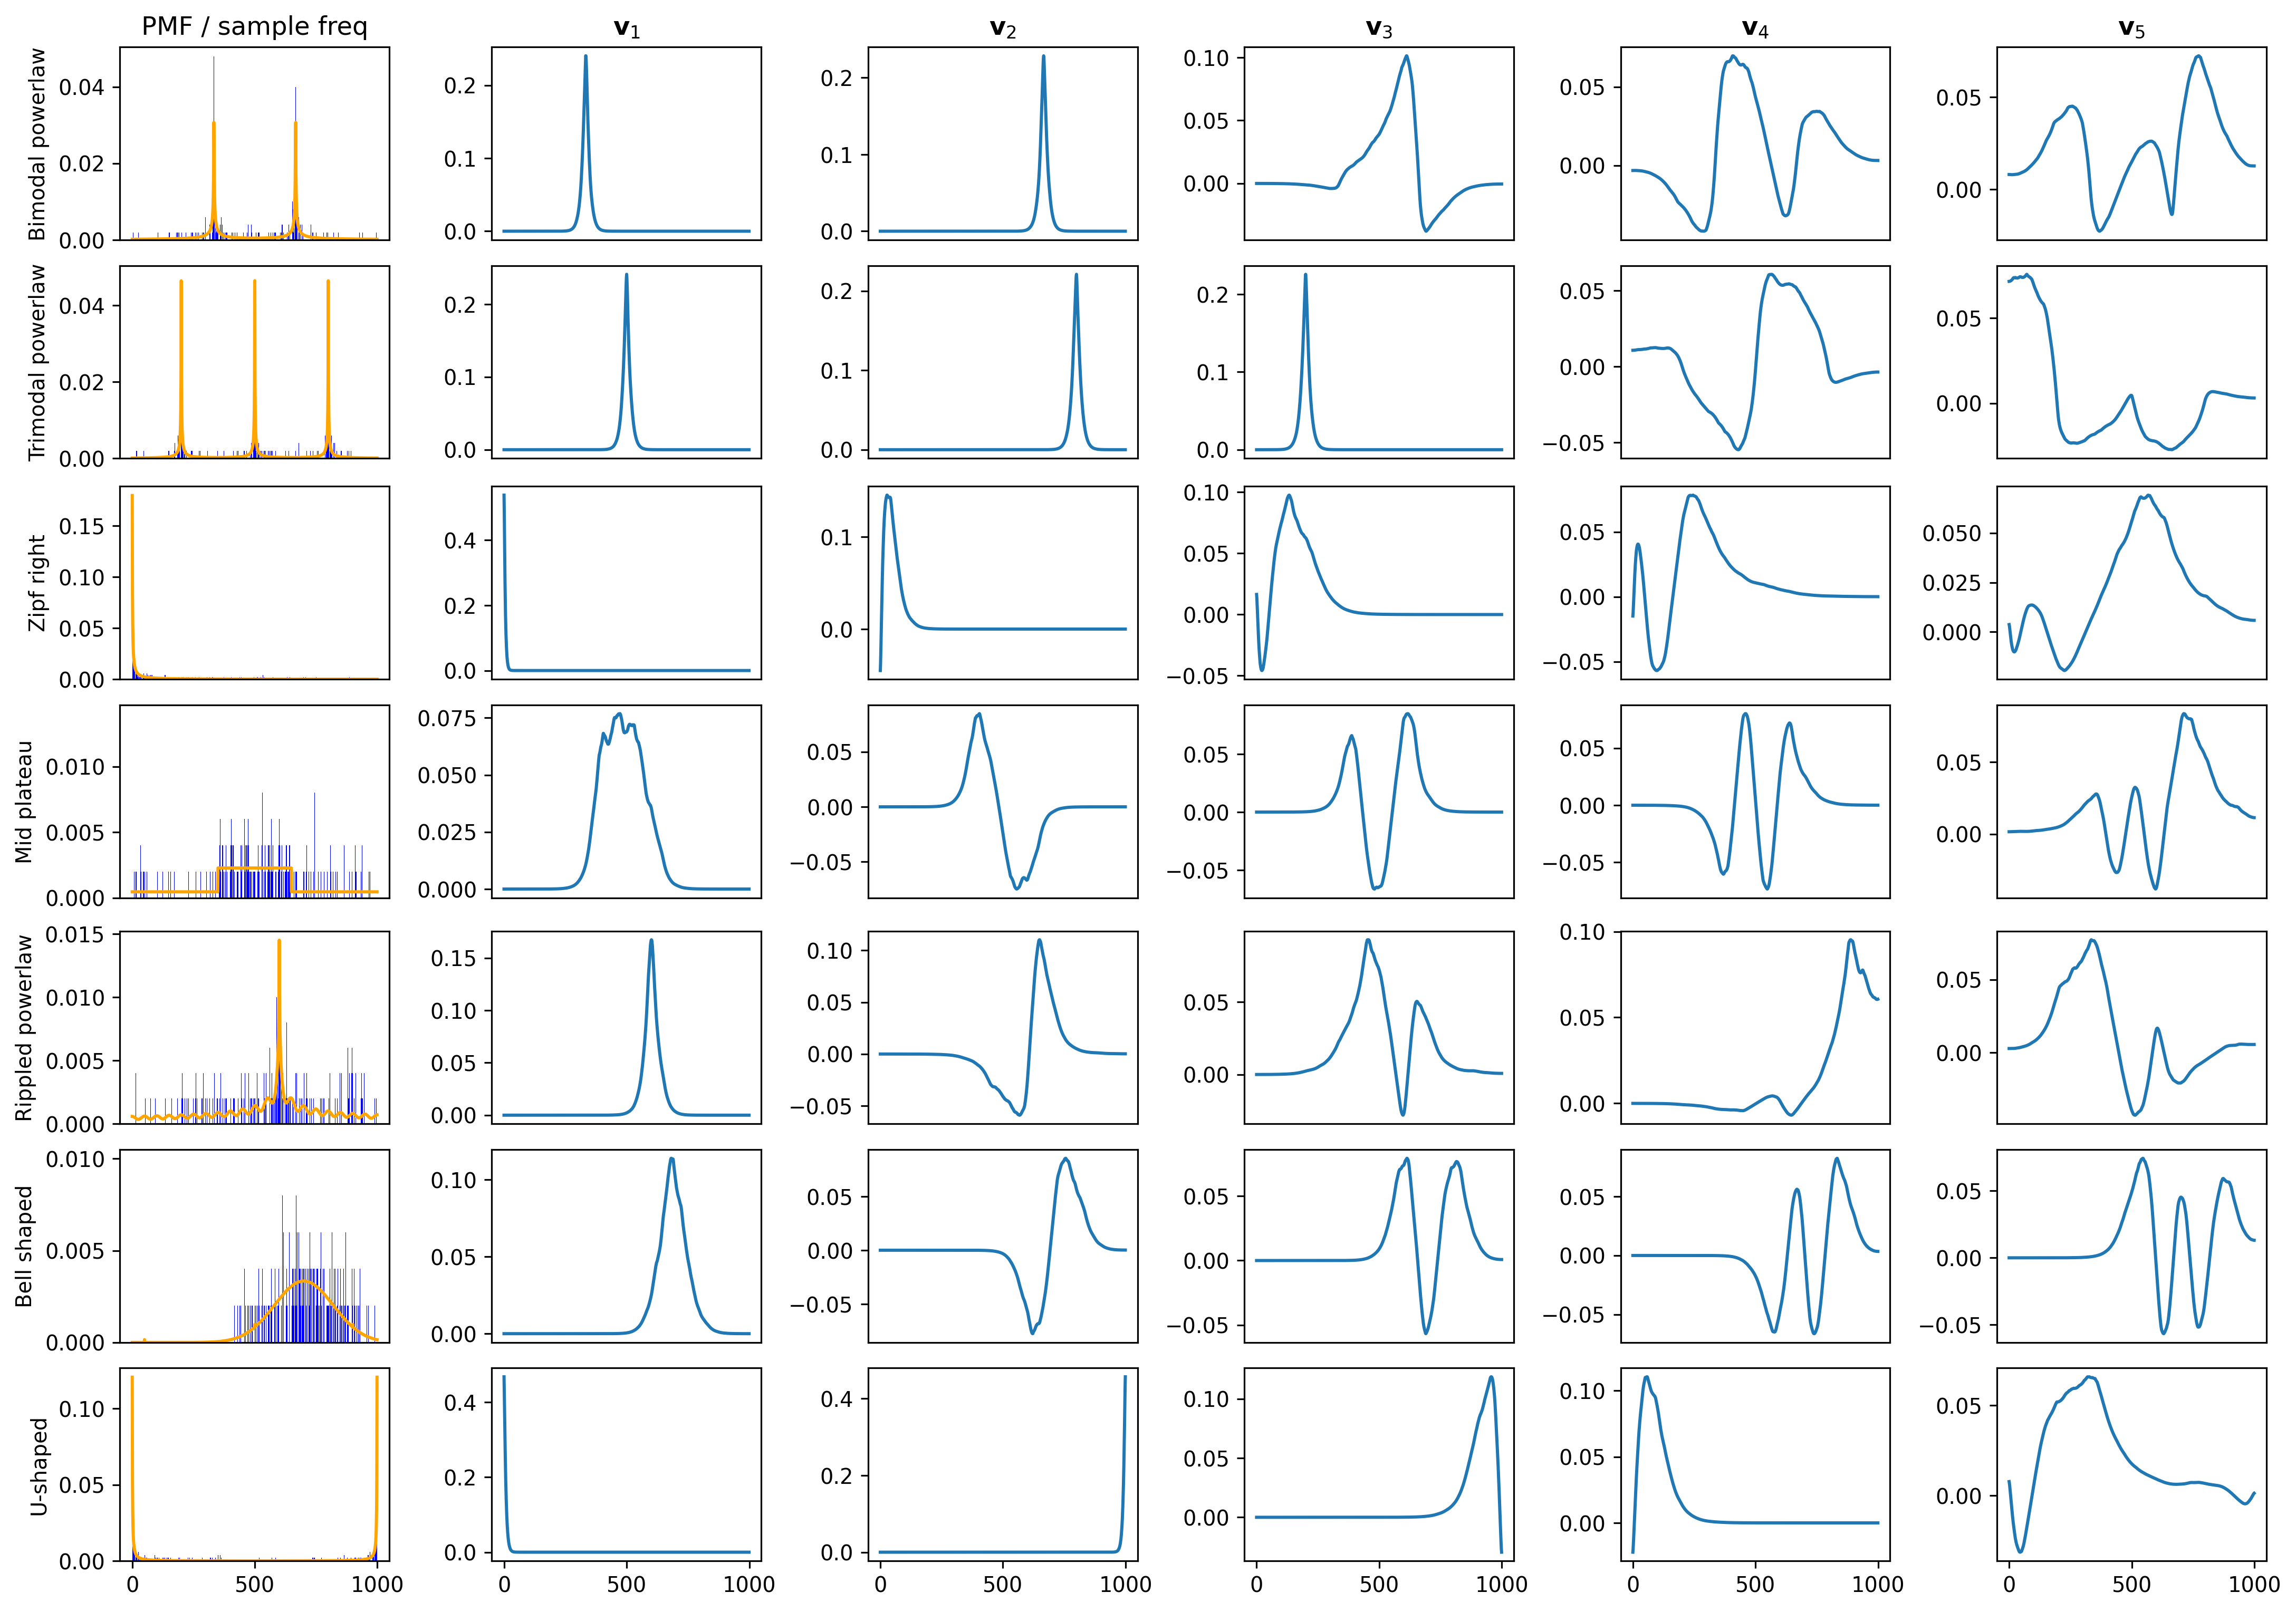
\includegraphics[width=\textwidth]{eigenvectors}
    \caption{PMFs, samples, and eigenvectors. The left-most column has the true PMF supported on $0, 1, \dots, 999$ in orange, and empirical frequencies $\vp$ obtained from 500 samples in blue. The next columns depict the first five eigenvectors of $\mL - \diag(\vp)$.}
    \label{fig:eigenvectors}
\end{figure}

We do realize that different data-fitting terms, such as $\langle \vx, \vp \rangle$ or $\langle \vx, \vp \rangle^2$ appear more natural. These terms that consider similarity between $\vx$ and $\vp$ directly, and perhaps others, may appear better suited. In additionl, the first-order difference matrix above may not be the best way to approximate the ``derivative'' of our discrete signal, and better approximations exist \citep{semiclassical}. However, these do \emph{not} translate into one call to a fast symmetric tri-diagonal eigen-solver. This is a deliberate design decision we make in this work: we trade some quality for simplicity, speed, and reliability.

\Figref{fig:apx_synthetic_500} continues \figref{fig:eigenvectors}, and depicts the projections of the empirical frequencies onto the space spanned by the first $k$ eigenvectors, for various values of $k$ with 500 samples. As is apparent, the spiky shape of the heavy-tailed mixtures is nicely captured by the projection. In contrast, a bell-shaped distribution is poorly captured, even with 10 eigenvectors. A distribution with an abruptly changing PMF, the ``Mid plateau'', is a case when our method fails.

\begin{figure}[tbh]
    \centering
    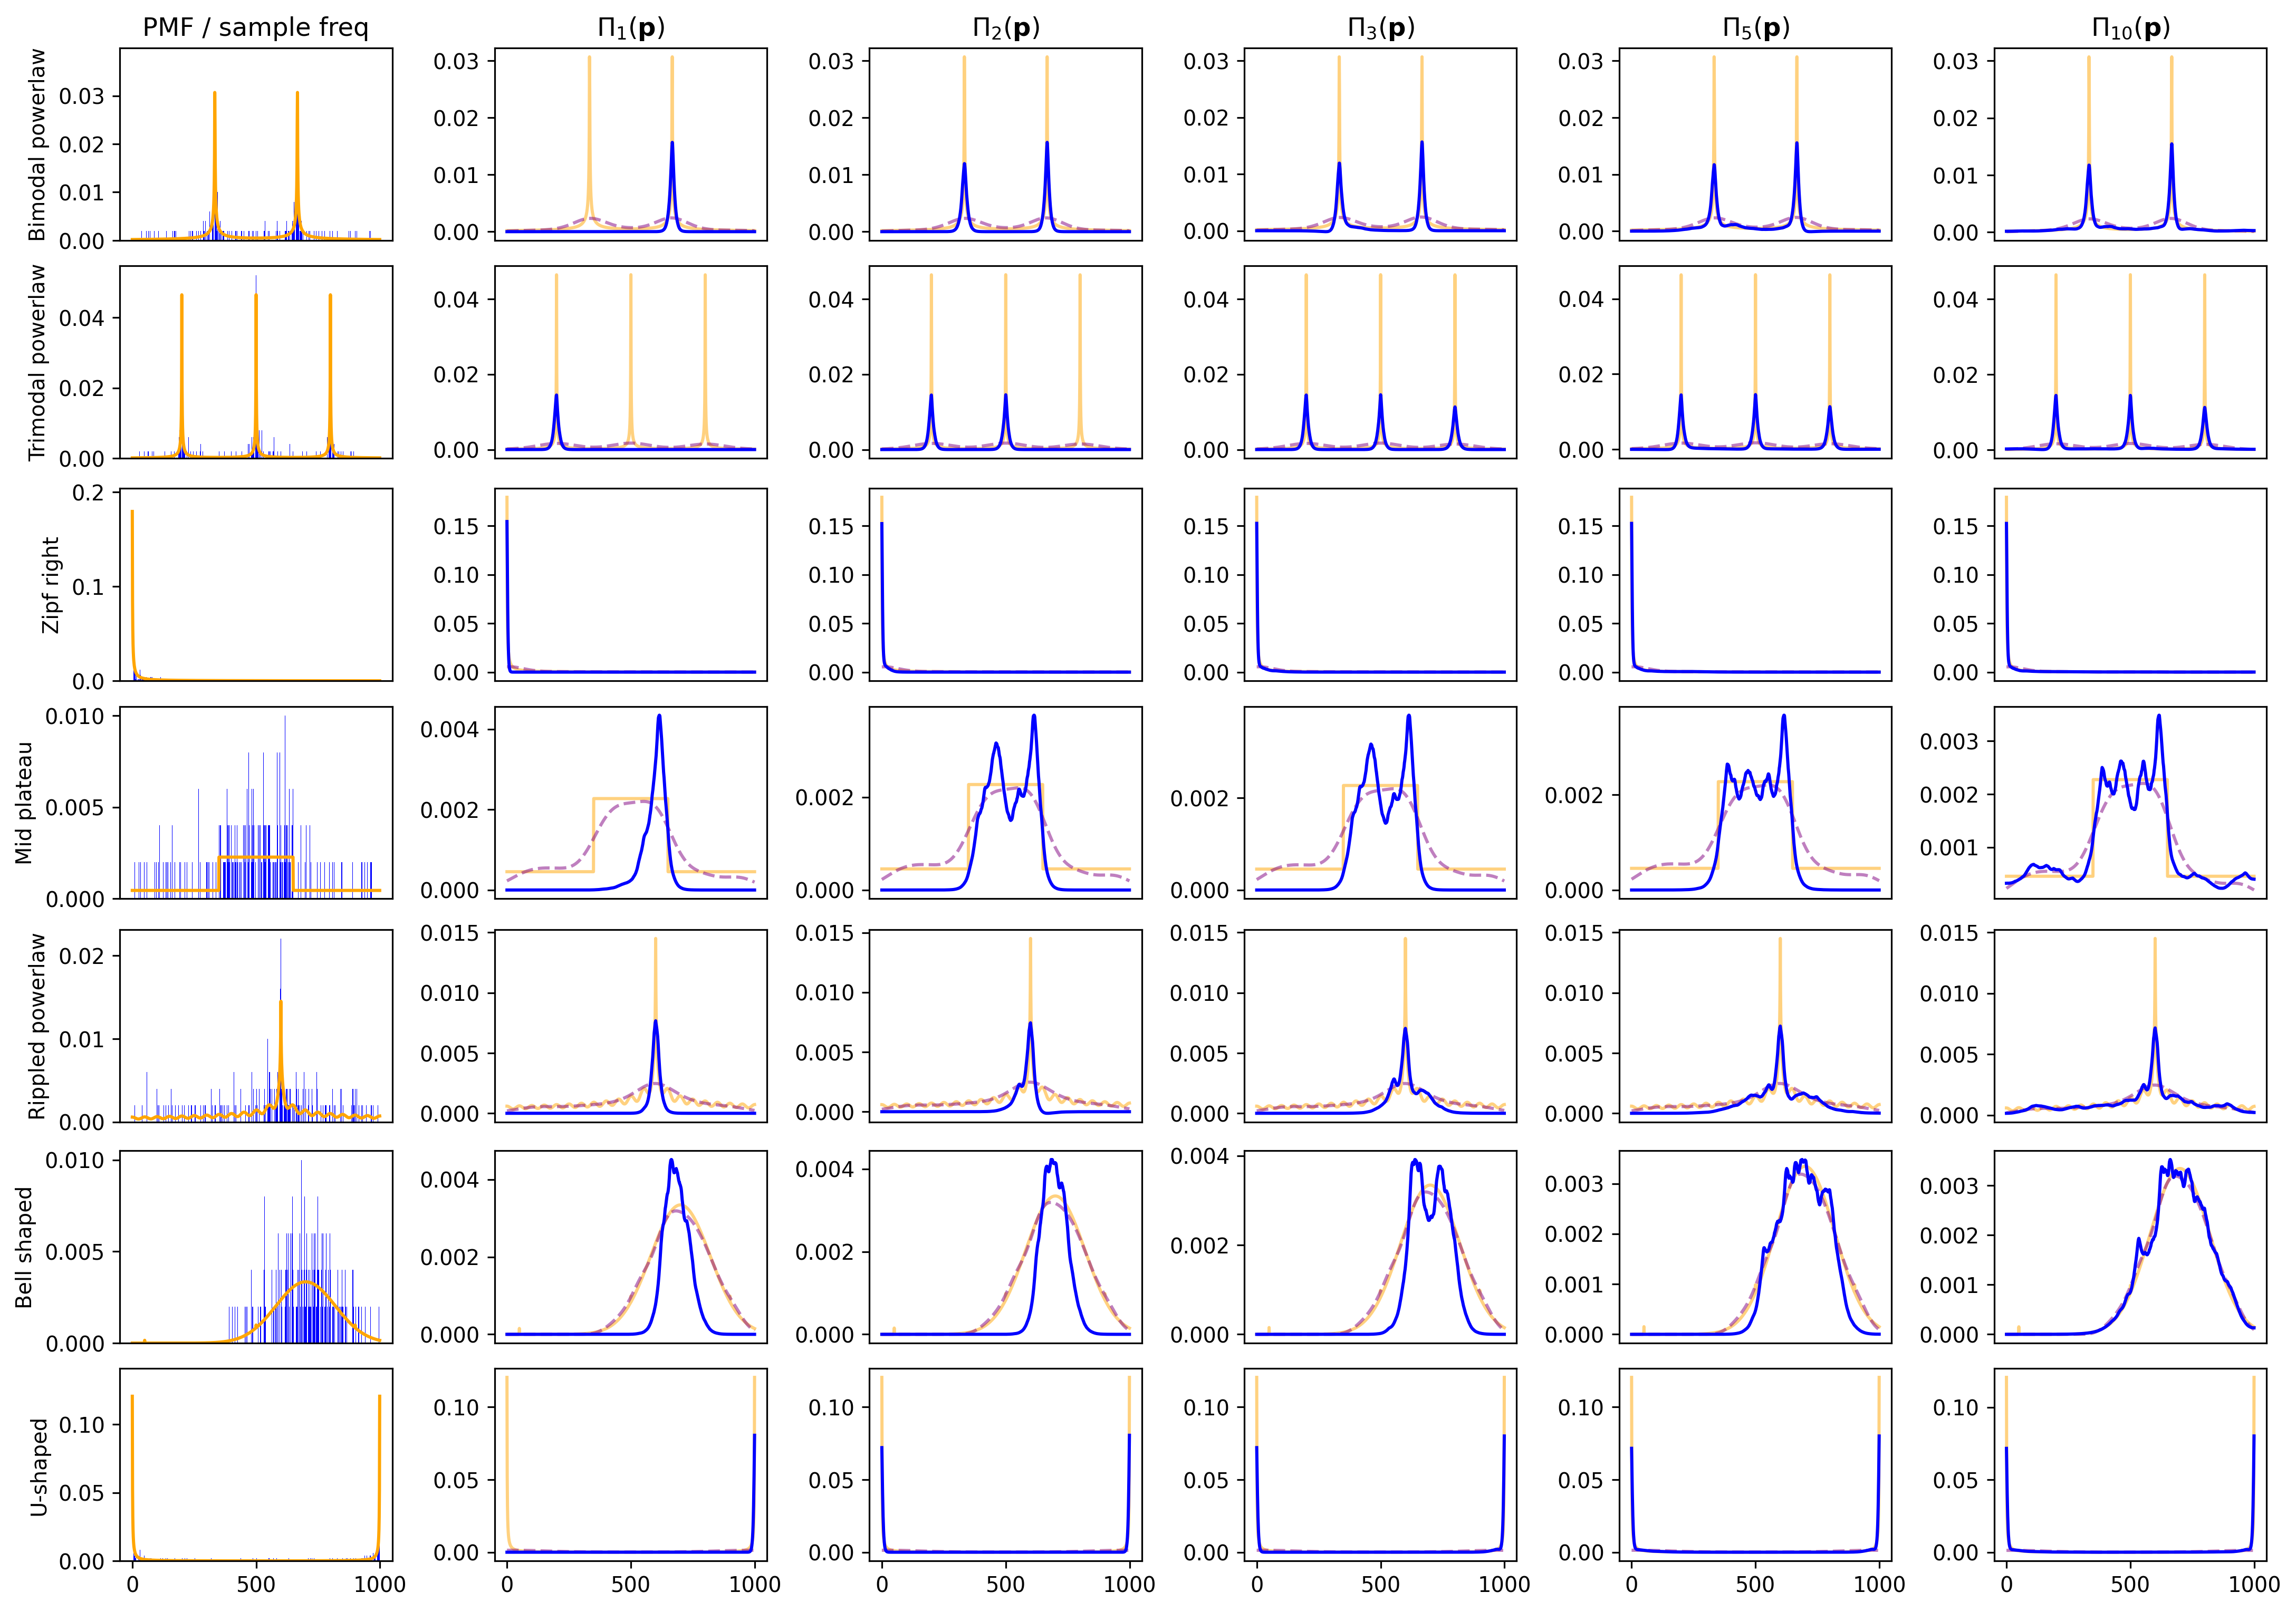
\includegraphics[width=\textwidth]{proj_500_samples}
    \caption{The projections of the empirical frequencies stemming from 500 samples from $\{0, 1, \dots, 4999\}$ onto the first $k$ eigenvectors of $\mL - \diag(\vp)$ for different values of $k$. Rows are various distribution shapes. The first column depicts the sample frequencies along with the true PMF. The next columns depict projections of this empirical frequency vector onto eigenspaces of increasing dimension in blue.}
    \label{fig:apx_synthetic_500}
\end{figure}

To appreciate how our method scales with various sample sizes, we plot the projection onto the first $k=10$ eigenvectors the empirical frequency vectors coming from increasingly large samples in \figref{fig:apx_sample_sizes}. The same behavior persists - the shape of spiky distributions is nicely captured even at small sample sizes. A bell-shaped distribution requires more samples to capture. And finally, our method is poorly suited in the case of an abruptly changing PMF, the ``Mid plateau''. 

\begin{figure}[tbh]
    \centering
    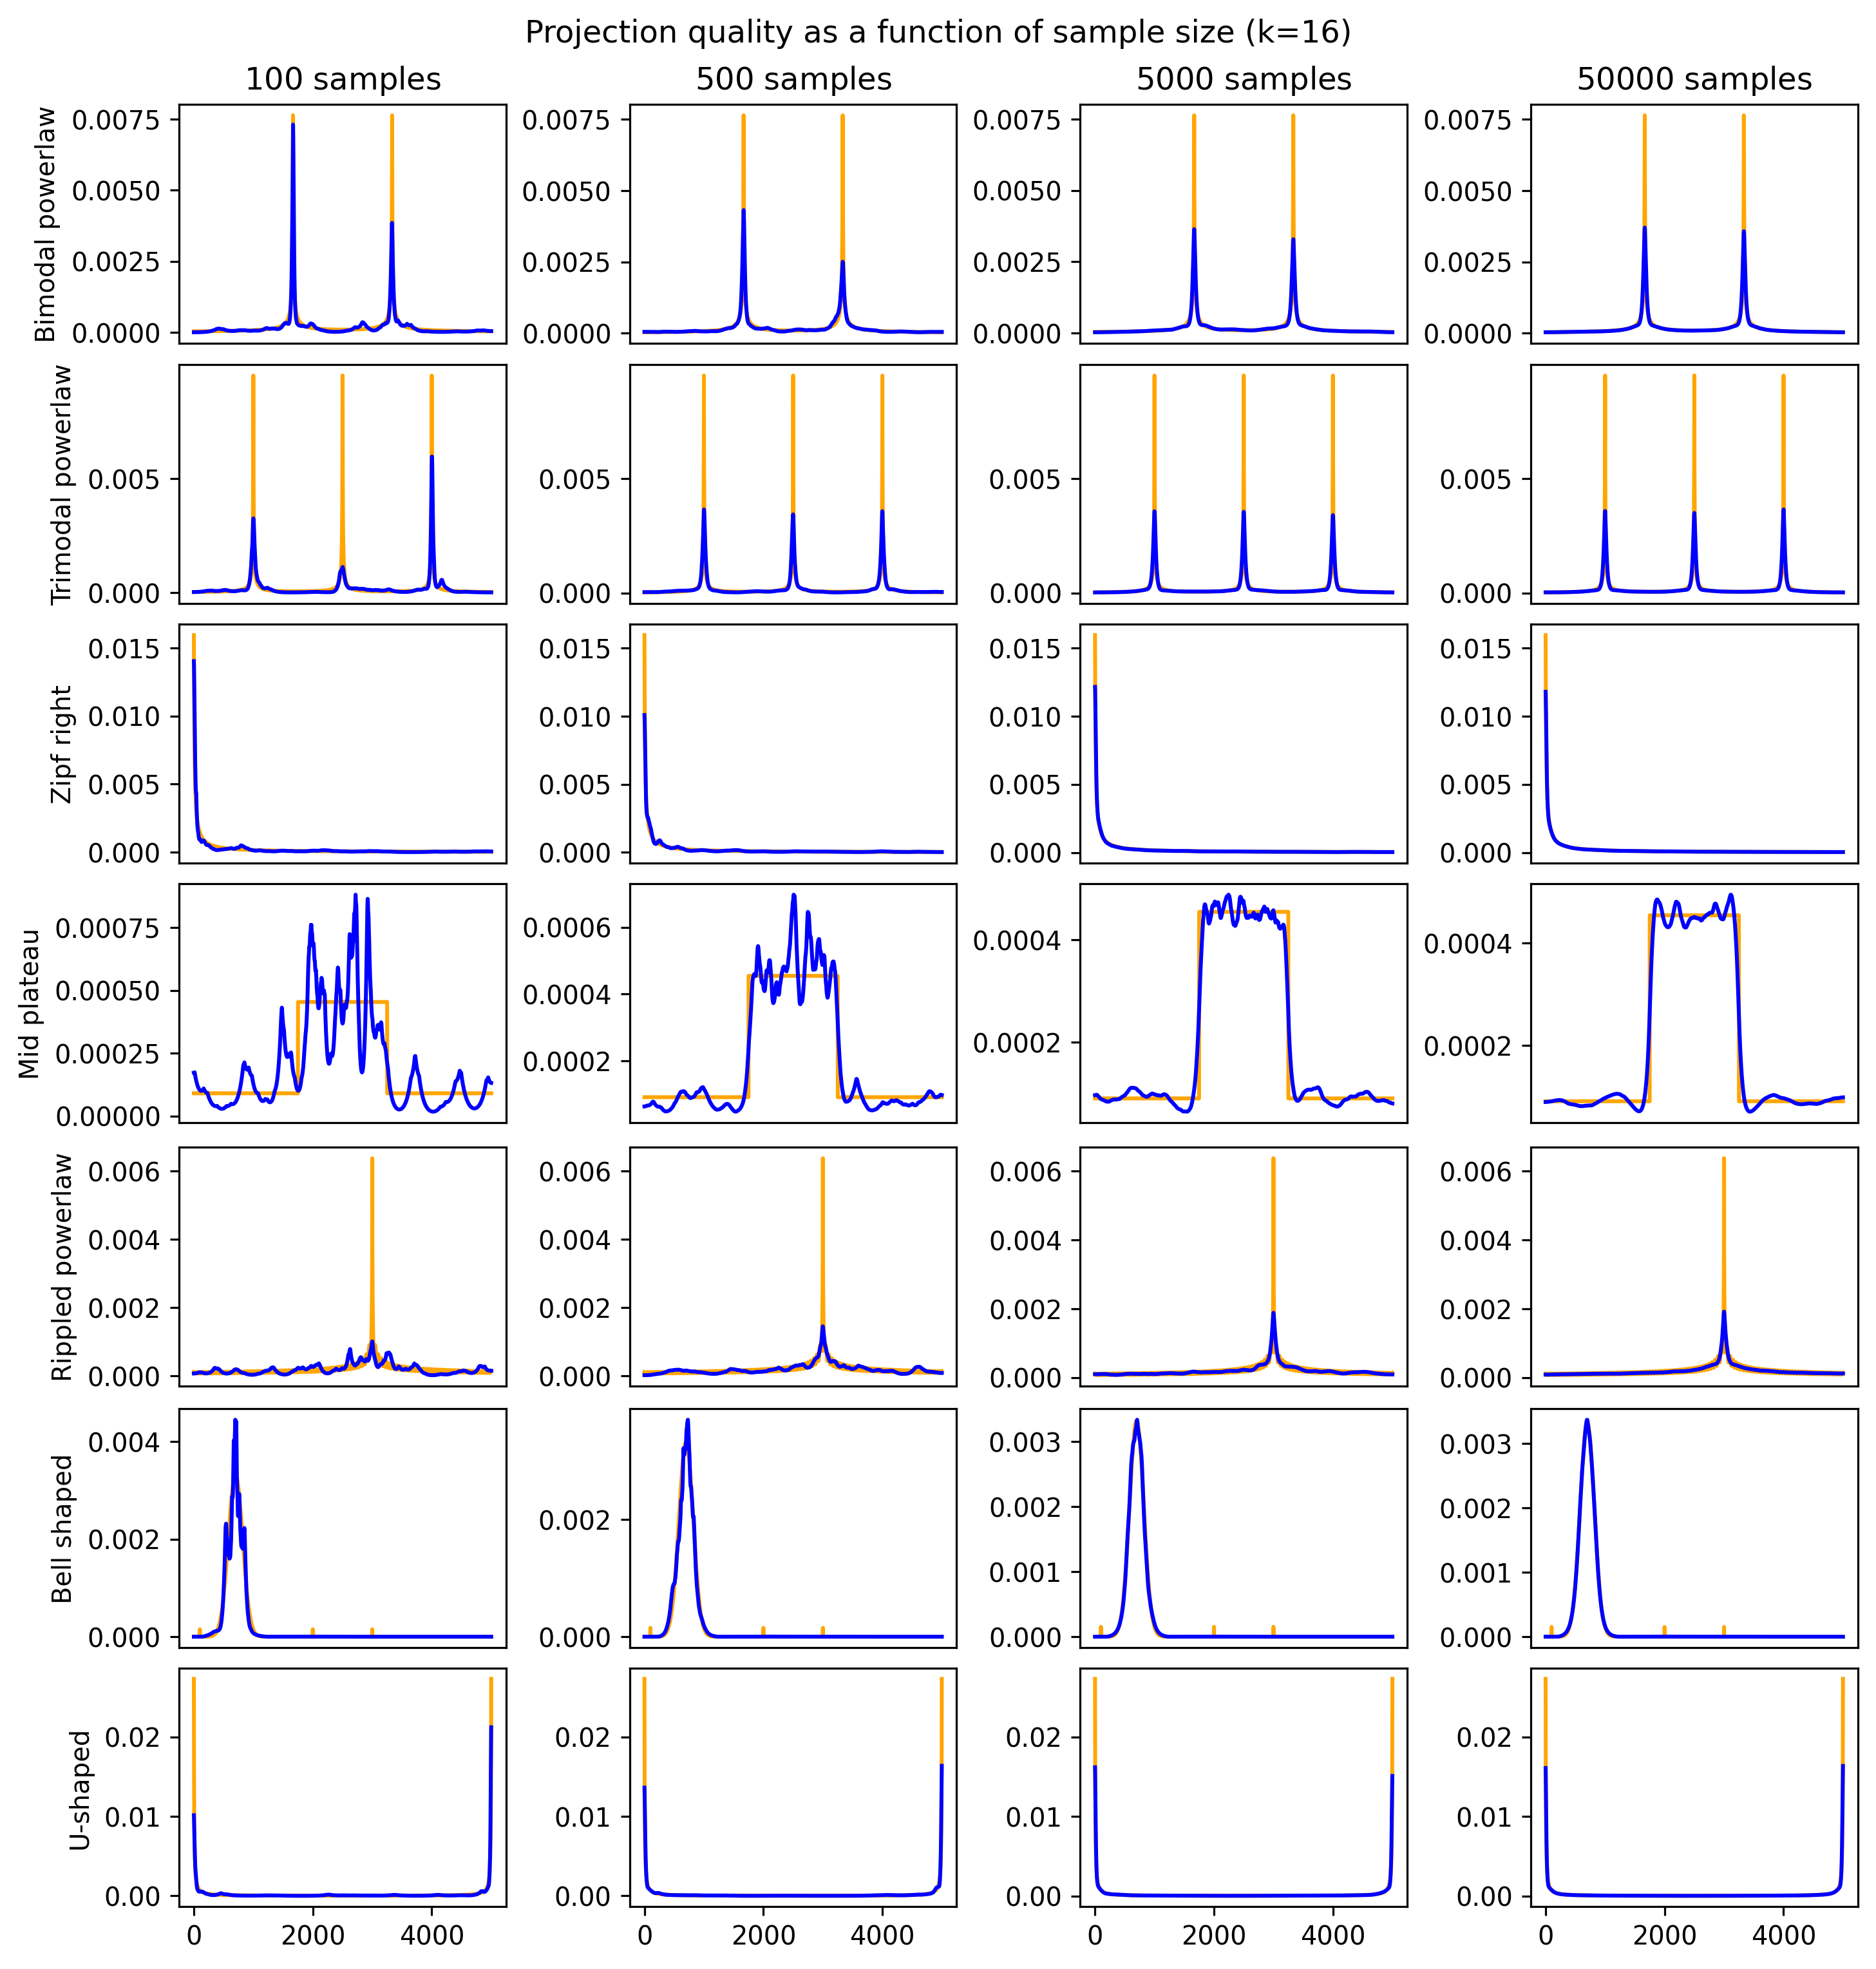
\includegraphics[width=\textwidth]{proj_diff_samples.png}
    \caption{The projections of the empirical histograms stemming from  samples from $\{0, 1, \dots, 4999\}$ of various sizes onto the first $k=16$ eigenvectors of $\mL - \diag(\vp)$. Rows are various distribution shapes. Columns represent sample sizes. Our method in blue, whereas the true density in yellow.}
    \label{fig:apx_sample_sizes}
\end{figure}

\section{Automated selection of the number of eigenvalues}
Since the entire spectrum of the matrix is an orthonormal basis, it can exactly represent the empirical frequency vector. Thus, using the subspace of just the first $k$ first eigenvectors is a form of regularization, where less eigenvectors correspond to stronger regularization. Intuitively, the more data we have, the less we may need to regularize. Indeed, looking again at \figref{fig:apx_sample_sizes} we can see that 16 eigenvectors appear to be too much for small samples. Thus, we need some technique to select the appropriate number $k$ of eigenvectors to use. Such a selection technique, if turns out to work well, also eliminates the need to specify $k$ and makes our method easier to use in practice.

We adopt a heuristic similar to \emph{logspline} described in \citet{StoneHansenKooperbergTruong1997} to select an upper bound on $k$. Then, we select the best $k$ based on a criterion similar to the Bayesian Information Criterion (BIC) \citep{schwarz1978estimating}. We do realize that cross-validation, and other techniques may yield more accurate PMF approximations, but again - we favor simplicity and speed over squeezing every ounce of approximation quality as a design decision, and demonstrate that it works reasonably well.

Concretely, our upper bound on the number of eigenvectors is identical to the \emph{logspline} upper bound on the number of spline knots, $K = \min(4 n^{1/5}, n / 4, N, 30)$, where $n$ is the number of observations in the sample, and $N$ is the number of unique values in the sample. For selecting the number of spline knots, logspline uses the Bayesian Information Criterion (BIC). 

Since our fitting procedure is a \emph{Euclidean projection onto an orthogonal basis}, rather than log-likelihood minimization, we cannot use BIC directly for estimating the expected error. Rather, we use the variant described in \citet{diggle_hall_orthogonal_selection}. Given an orthonormal basis $\mV = [\vv_1 \lvert \dots \rvert \vv_K]$ and an empirical frequency vector $\vp$ obtained from $n$ observations, first we compute
\begin{itemize}
    \item the projection coefficients $\vc = \mV^T \vp$,
    \item the basis 2nd-order moment $\vs^2 = (\mV \odot \mV)^T \vp$, where $\odot$ is the Hadamard product,
    \item estimated squared basis coefficients of the \emph{true} PMF $\bar{\vc}^2 = \frac{1}{n-1} \left[n \vc^2 -  \vs^2\right]_+$,
\end{itemize}
and then we compute the expected L2 error estimate of using just $m$ out of $K$ eigenvectors:
\[
\mathcal{E}(m) = \frac{1}{n}\sum_{k=1}^m (s_k^2 - \bar{c}_k^2) + \sum_{k=m+1}^K \bar{c}_k^2.
\]
Consequently, we use $k_{\mathrm{best}} = \argmin_{1 \leq m \leq K} \mathcal{E}(m)$ eigenvectors. Note, that the vectors $\vc$, $\vs^2$, and $\bar{\vc}^2$ are computed \emph{once}, and then $k$ is selected based on these vectors. Explaining the somewhat ``magic'' appearance of the above method is out of the scope of this paper, but we refer readers to \citet{diggle_hall_orthogonal_selection} for its derivation.

Even with the above automated selection of $k$, the entire algorithm, fits in a short snippet of Python code:
\begin{pycode}
def hist_estimator(samples):
    # compute empirical frequencies (assume support is [0 ... MAX])
    n = len(samples)
    p = np.bincount(samples, minlength=np.max(samples)).astype(float) / n

    # estimate upper bound on the number of eigenvectors - based on the logspline heuristic
    N = np.count_nonzero(p)
    K = int(math.ceil(min(4 * n ** (1/5), n / 4, N, 30)))

    # compute the first K eigenvectors
    diag = np.r_[1, np.full(p.size - 2, 2), 1] - p
    off_diag = np.full(p.size - 1, -1)
    _, V = scipy.linalg.eigh_tridiagonal(diag, off_diag, select="i", select_range=(0, k - 1))

    # estimate L2 error
    coefs = V.T @ p
    raw_2nd_moment = np.square(V).T @ p
    true_coef_sq_est = (
        np.maximum(0, n / (n - 1) * np.square(coefs) - 1 / (n - 1) * raw_2nd_moment) if n > 1
        else np.zeros_like(coefs)
    )
    err_estimate = (
        np.cumsum(raw_2nd_moment - true_coef_sq_est) / n +
        (np.cumsum(coef_sq_unbiased[::-1])[::-1] - coef_sq_unbiased)
    )

    # use k_best eigenvectors, and normalize
    k_best = np.argmin(risk_estimate) + 1
    u = V[:, :k_best] @ coefs[:k_best]
    return np.maximum(0, u) / np.sum(np.maximum(0,u))
\end{pycode}

In \figref{fig:performance_comparison_synthetic} we compare the algorithm algorithm to logspline, and Gaussian kernel-density estimation as availabe in SciPy \citep{scipy} with automatic bandwidth selection. Our objective is observing fitting quality \emph{without} human intervention or tuning. We can see that our method indeed performs well in the heavy-tailed setting, as does logspline. Our method is competitive with logspline, each having its advantages in different settings and different sample sizes. Out of these examples, Gaussian kernel density estimation fits well only in the bell-shaped case. As predicted, our method does \emph{not} perform well on the ``Mid plateau'' PMF, in contrast to both logspline and kernel density estimation, that despite low fitting quality, perform quite gracefully.

\begin{figure}[tbh]
    \centering
    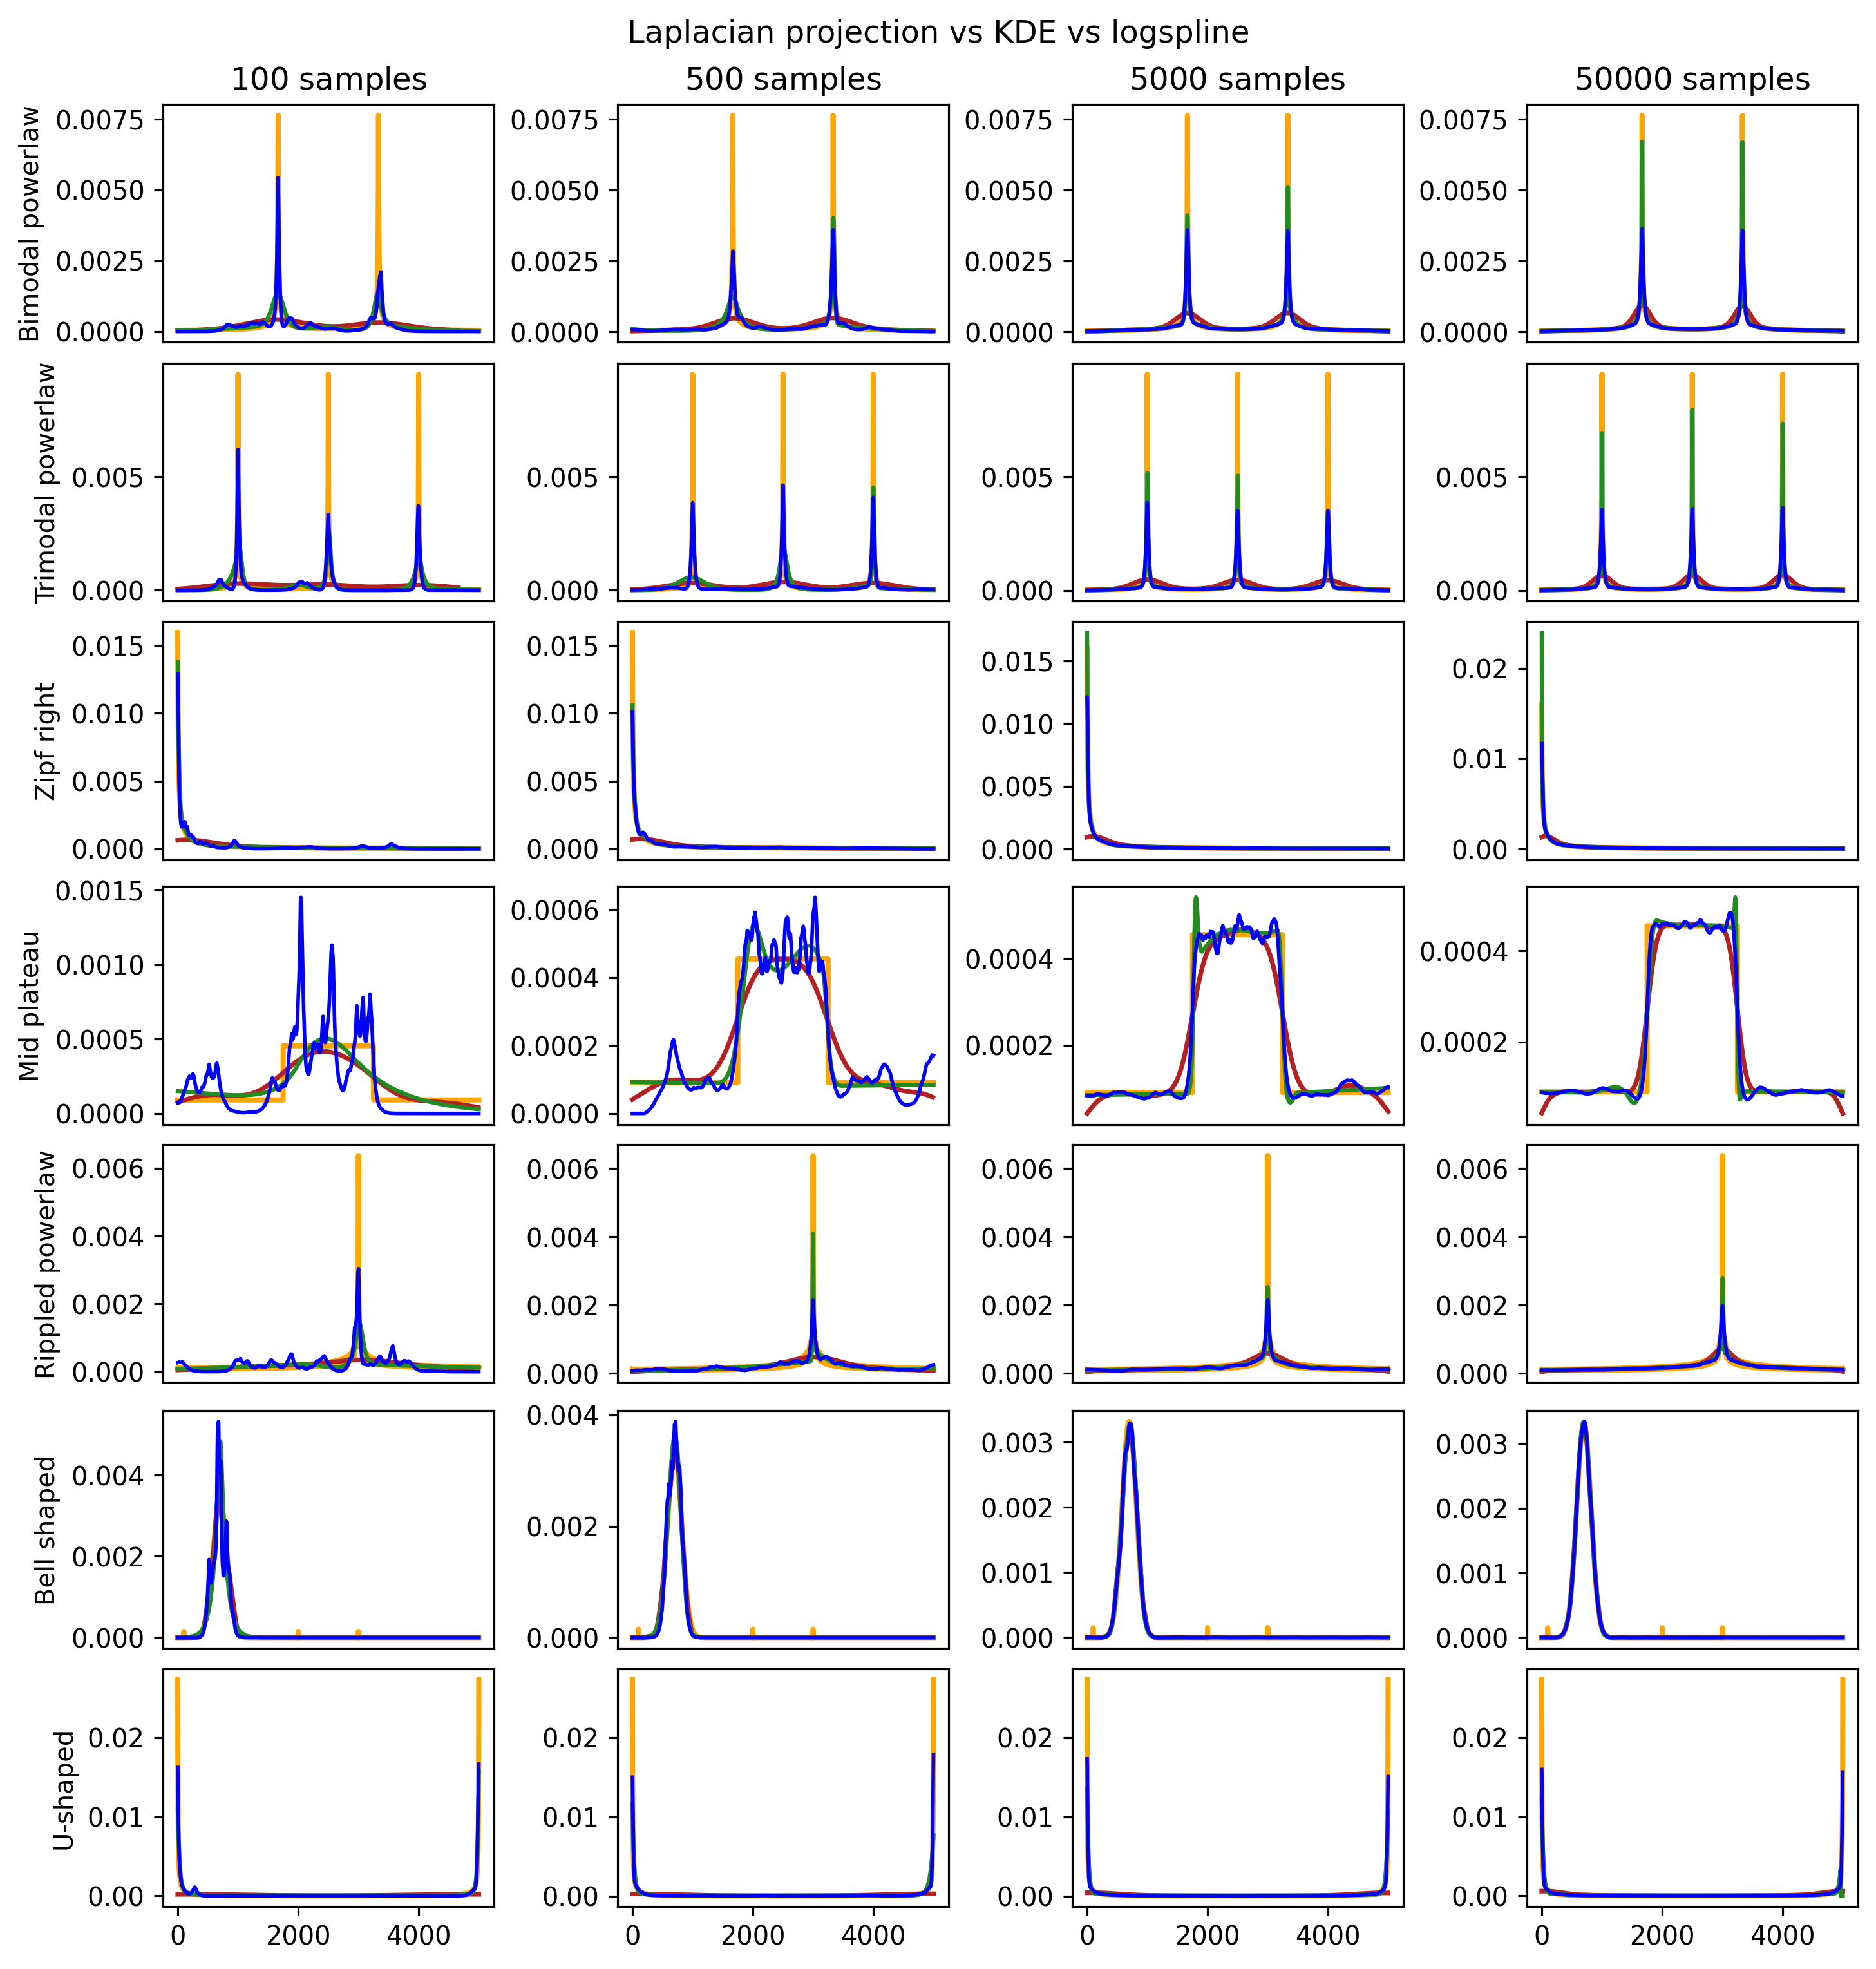
\includegraphics[width=\textwidth]{performance_synthetic_comparison.png}
    \caption{Fits obtained for different sample sizes with out method (blue), Gaussian kernel-density estimate (red), and logspline (green). The true PMF is in yellow. Rows are different distributions, whereas columns are different sample sizes.}
    \label{fig:performance_comparison_synthetic}
\end{figure}

The above error estimate, despite being just an upper bound, also implicitly assumes that the basis is chosen a-priori, independent of the data. This is not the case in our method - the columns of $\mV$ heavily depend on the data by construction of the eigen-problem. Thus, this method is just a heuristic. But again,  we make a conscious design decision of using a method we know to be sub-optimal, while gaining simplicity and speed. As we just demonstrated on the synthetic data, and in the next section on real data - this turns out to work reasonably well in practice.

\section{Testing on real data}
We use the \emph{spambase} dataset \citep{spambase_94} for spam classification, due to a large number of heavy-tailed numerical columns representing token frequencies, letting us test our method in different settings. All frequencies as multiplied by $1000$ and rounded, to obtain integers as our method expects. We also use the bank marketing dataset \citep{bank_marketing_222} that has only \emph{one} numerical column, the bank account balance, but has a relatively large number of rows that let us test our method with various sample sizes.

Practical real-world numerical features tend to be both \emph{zero-inflated} and \emph{heavy tailed}. This is also the case with our two data-sets. We assume the zero inflation is dealt with separately, by estimating the probability of each feature being zero, and obtaining a separate PMF estimate assuming it is nonzero. Thus, for both datasets, we discard zero samples and test our methods on the non-zero samples.

In \figref{fig:spambase} we plot PMF estimates for all the feature columns in the data-set using our method (with automated selection of $k$), logspline, and Gaussian kernel density estimator. We can see that the kernel density estimator fails to produce a reasonable estimate for many columns, such as the \texttt{word\_freq\_report},  \texttt{word\_freq\_free}, and others. logspline and our method are quite competitive, but slightly different. While logspline fits even small peaks, our method assumes them to be just noise. We can also see that for some features logspline produced somewhat un-expected estimates, such as the \texttt{char\_freq\_;}, \texttt{char\_freq\_(}, and \texttt{char\_freq\_\#} features. 

One interesting observation is that for  one feature is missing a logspline estimate altogether -  \texttt{capital\_run\_length\_average} feature. This is because logspline \emph{failed to converge}, and threw an exception with convergence failure as its message. It turns out that failure to converge, even if not common, still may happen due to the fitting procedure's reliance on numerical optimization methods that require tuning. Thus, even though it may perform well for many problem instances, logspline becomes less useful for automated pipelines that are required to work reliably without human intervention.

\begin{figure}
    \centering
    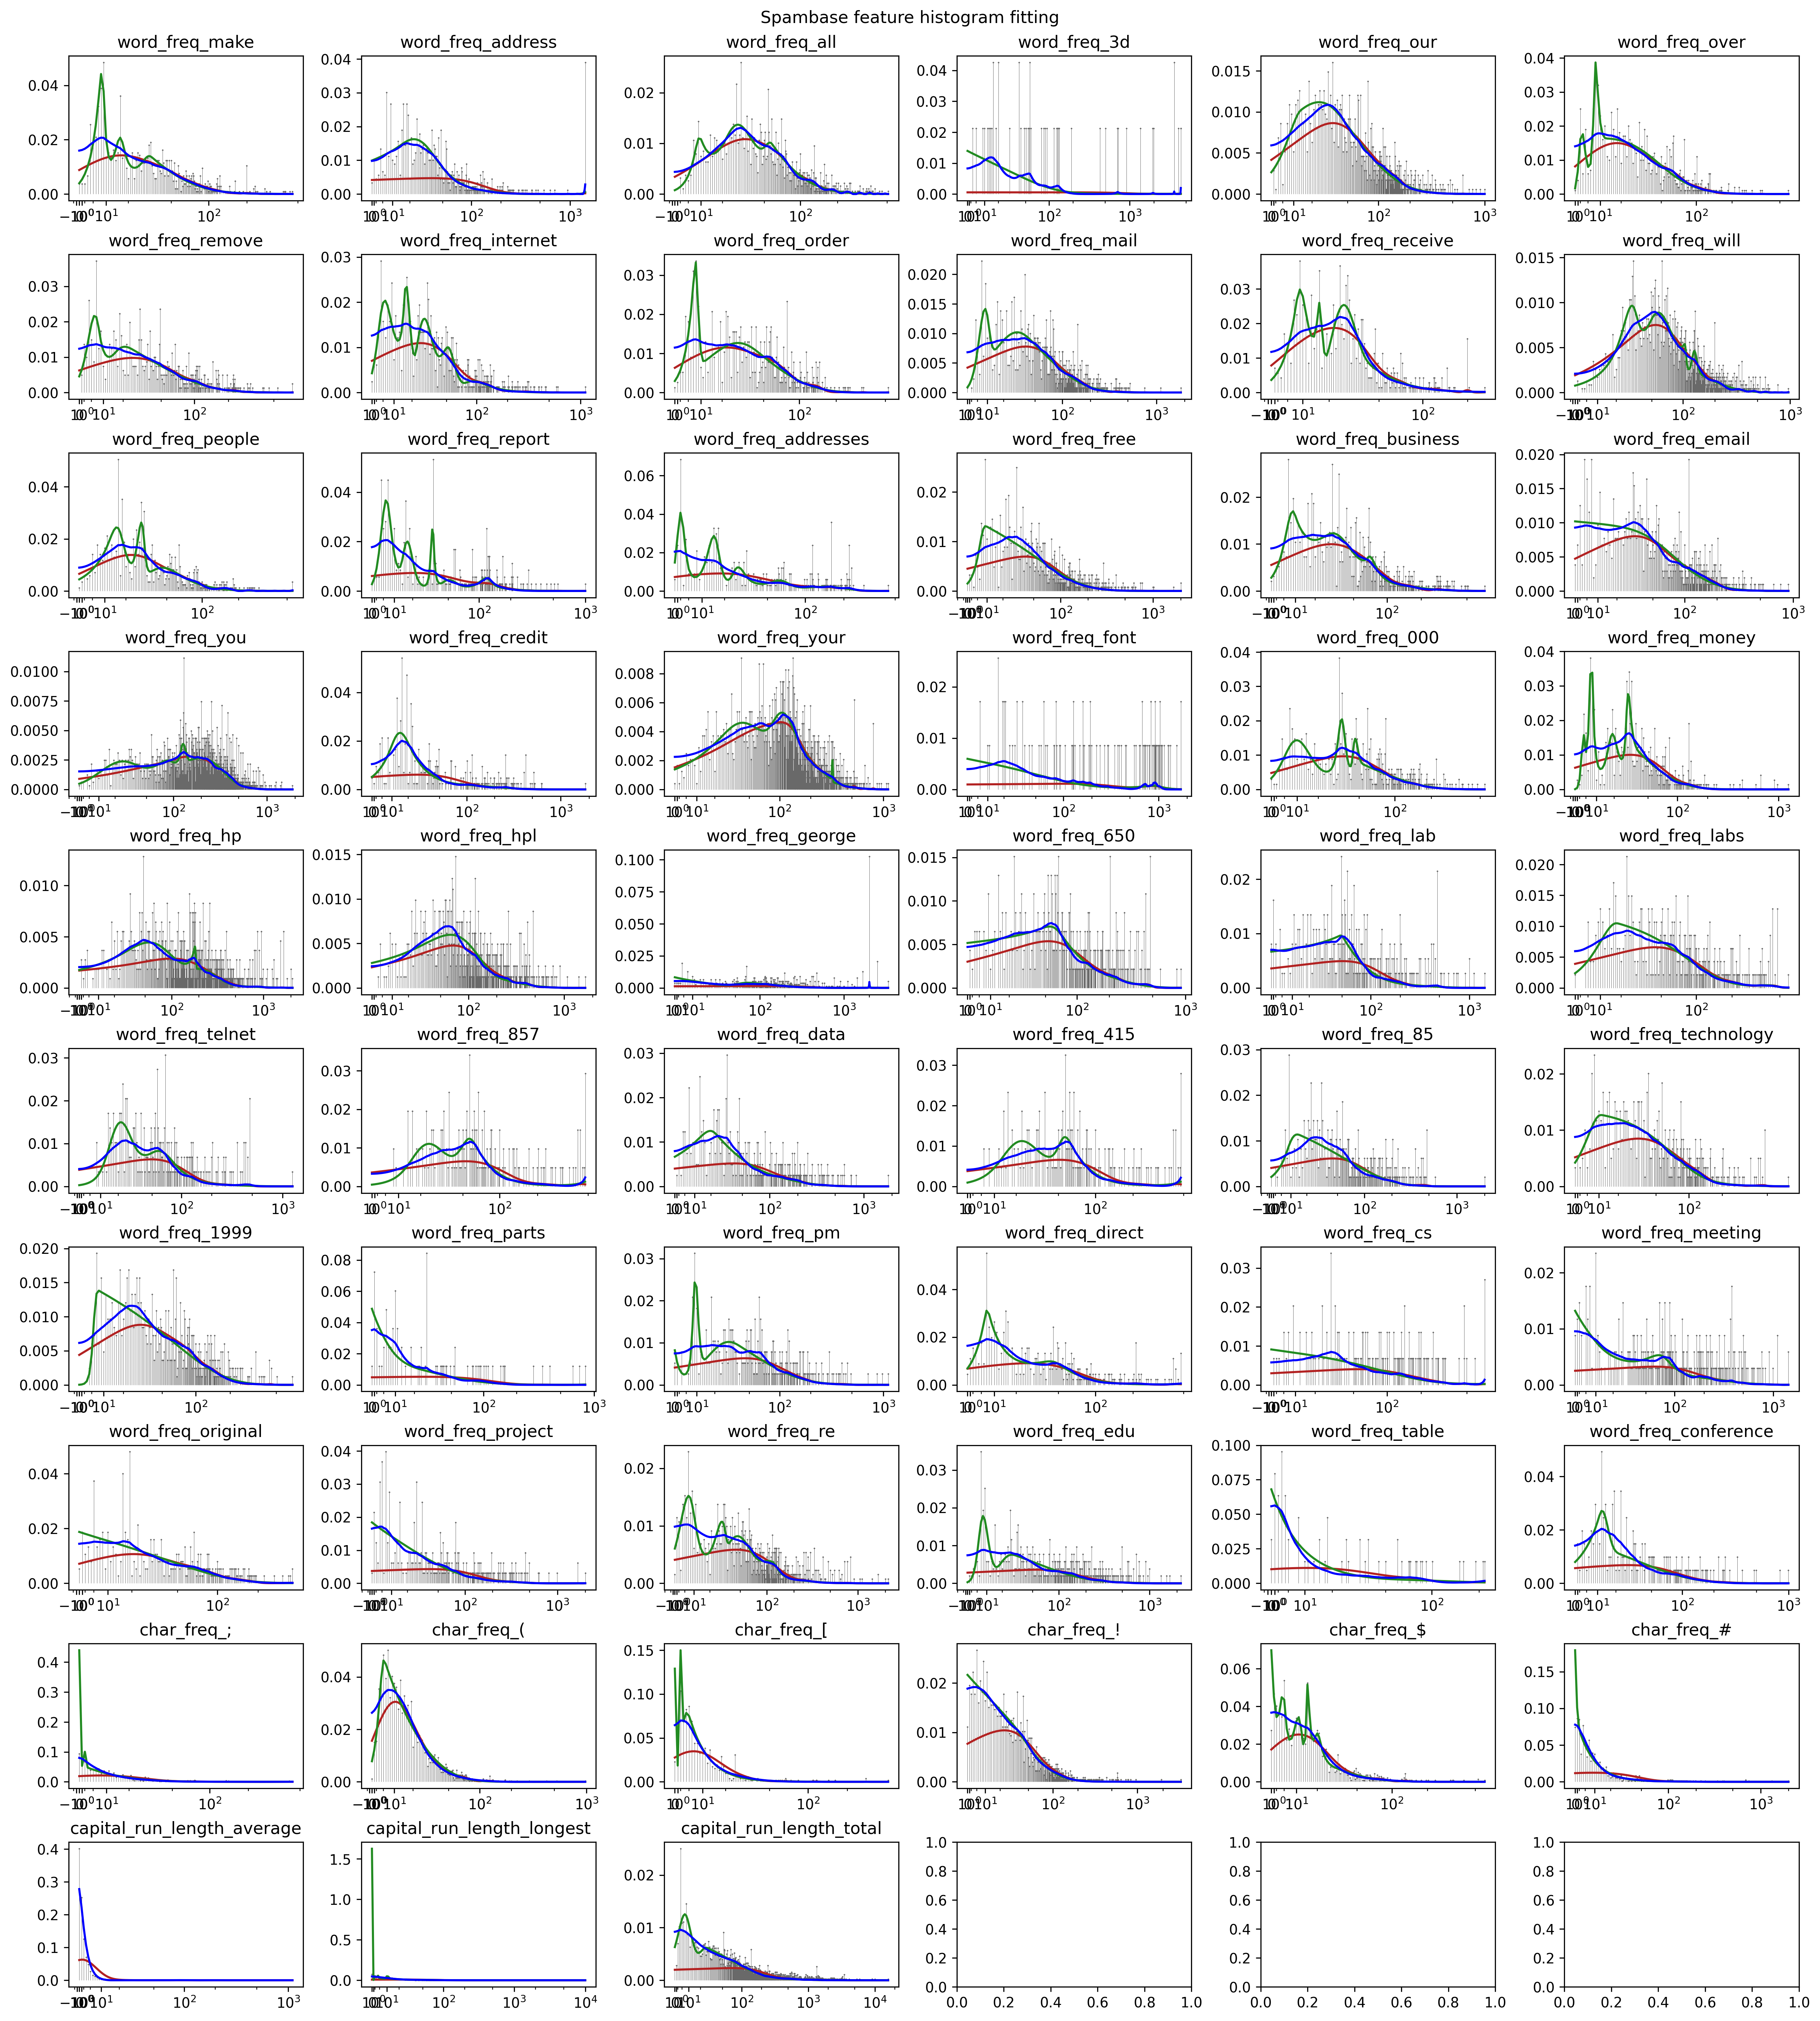
\includegraphics[width=\textwidth]{spambase.png}
    \caption{Empirical frequencies (gray) and PMF estimates for columns of the spambase dataset. Gaussian kernel-density estimator in red, logpline in green, and our method in blue.}
    \label{fig:spambase}
\end{figure}

For the bank marketing data-set, the balance is already an integer, but can be negative. To apply our method, we first shifted the non-zero observations by the minimum balance, but plot the obtained PMF in the original coordinate system to make all methods comparable. In \figref{fig:bank_balance} we can see our method, logspline, and kernel-density estimation given various sample-sizes obtained by subsampling the balance column uniformly at random. Again, the kernel-density estimator struggles, whereas our method is competitive with, and almost identical to.

\begin{figure}
    \centering
    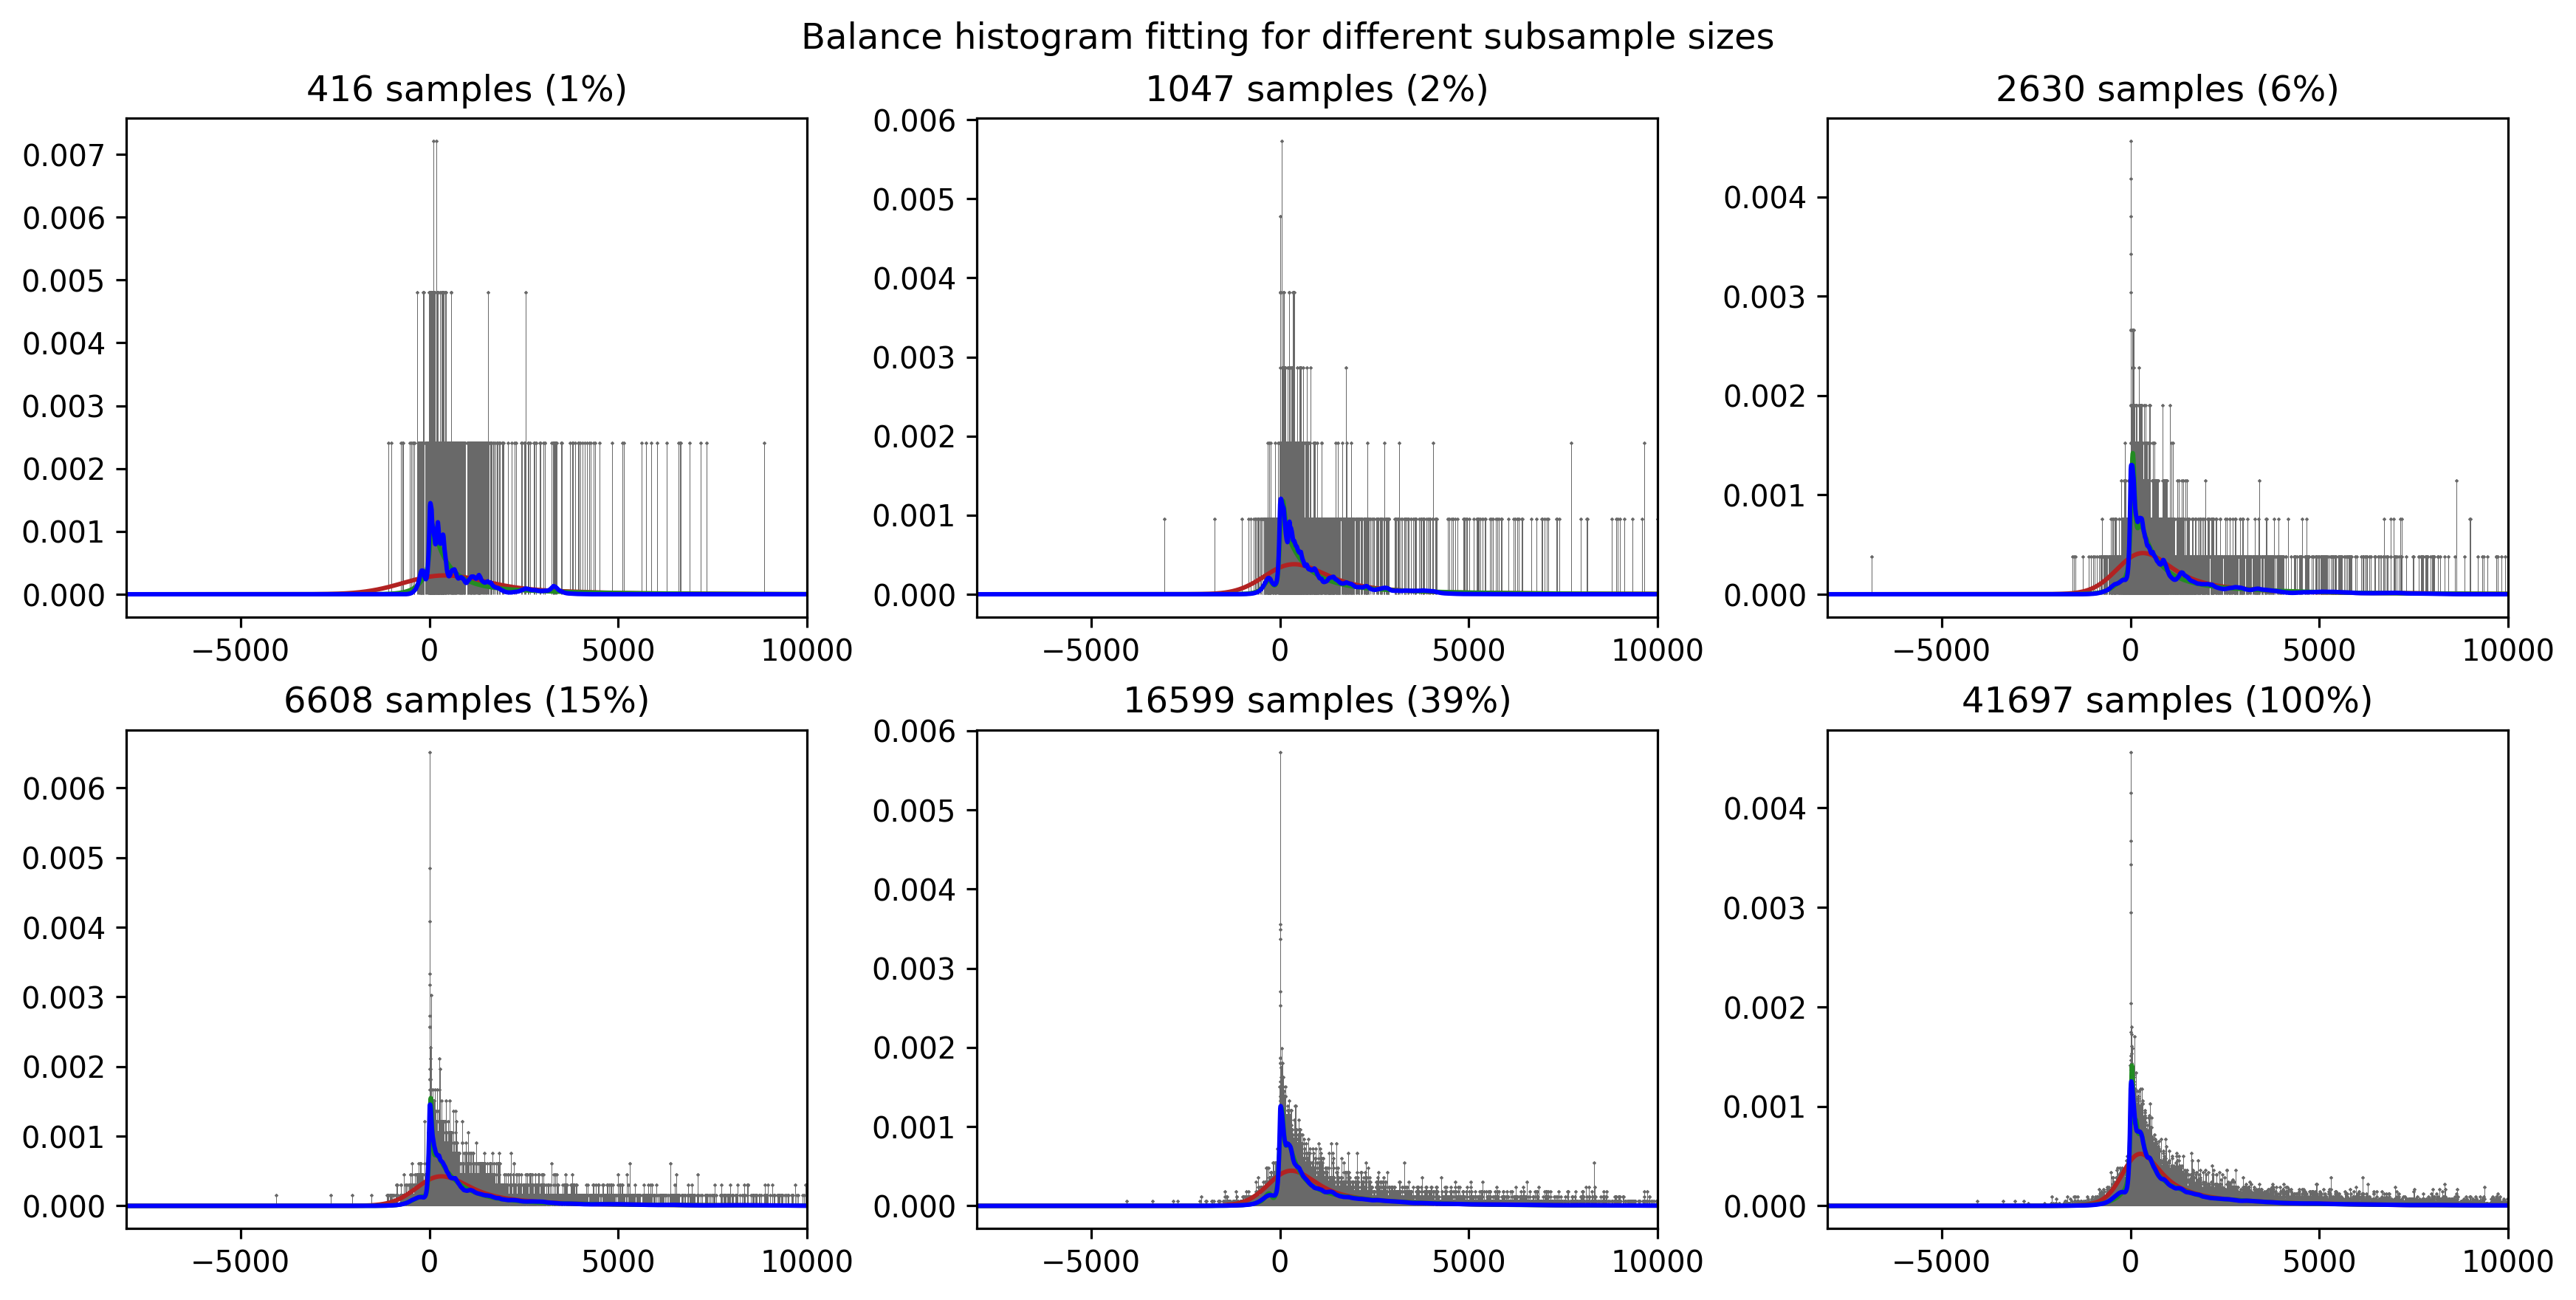
\includegraphics[width=\linewidth]{bank_balance.png}
    \caption{Empirical frequencies (gray) and PMF estimates for balance column of the bank marketing dataset. Gaussian kernel-density estimator in red, logpline in green, and our method in blue.}
    \label{fig:bank_balance}
\end{figure}


\section{Summary and discussion}
The method we proposed in this paper is simple, fast, and reliable, with many design decisions made to make sure it is that way. Its main competitor, logspline, makes a special effort to insert spline knots (break-points of a piece-wise polynomial function) at the right place to model the changing curvature of the distribution, whereas our method is adaptive to the data by design through the construction of the appropriate eigenproblem. 

The remarks spread throughout the paper suggest that better variants of our method can be obtained, such as different perturbation than $-\diag(p)$ which may not lead to a tridiagonal eigen-problem, or to an eigen-problem at all; perhaps a  different smoothness term than $\vx^T \mL \vx$ will yield a better method; better $k$ selection can be devised using cross-validation; and perhaps, even a better logspline-style method can be obtained by using our method as a "first-phase" to identify the knot placement regions. But these more advanced techniques are out out the scope of this work. Our aim was showing that projection onto a data-dependent basis, coupled with a simple model selection strategy work reasonably well for this problem.

It is our hope that the idea of using eigen-problems to obtain a data-adaptive representation bases, by interpreting them as the standard \emph{fitting term} + \emph{regularizer} minimization problem, becomes useful to our readers in other domains. In fact, this was one the reasons for the way we chose to present the content of this paper.

\bibliography{tmlr}
\bibliographystyle{tmlr}


\end{document}
